\documentclass{beamer}

\usepackage[utf8]{inputenc}
\usetheme[compress]{Dresden}
\setbeamertemplate{navigation symbols}{}    % remove navigation symbols from footer
\renewcommand\mathfamilydefault{\rmdefault} % set normal math fonts, there is a different default

% very "hacky" addition of page number to Dresden theme
\setbeamertemplate{footline}%{miniframes theme}
{%
    \begin{beamercolorbox}[colsep=1.5pt]{upper separation line foot}
    \end{beamercolorbox}
    \begin{beamercolorbox}[ht=2.5ex,dp=1.125ex,leftskip=.3cm,rightskip=.3cm plus1fil]{author in head/foot}%
        \leavevmode{\usebeamerfont{author in head/foot}\insertshortauthor}%
        \hfill%
        {\usebeamerfont{institute in head/foot}\usebeamercolor[fg]{institute in head/foot}\insertshortinstitute}%
    \end{beamercolorbox}%
    \begin{beamercolorbox}[ht=2.5ex,dp=1.125ex,leftskip=.3cm,rightskip=.3cm plus1fil]{title in head/foot}%
        {\usebeamerfont{title in head/foot}\insertshorttitle} \hfill     \insertframenumber%
    \end{beamercolorbox}%
    \begin{beamercolorbox}[colsep=1.5pt]{lower separation line foot}
    \end{beamercolorbox}
}

% very "hacky" change of footnote size
\setbeamertemplate{footnote}{%
  \tiny%
  \parindent 1em\noindent%
  \raggedright
  \hbox to 1.8em{\hfil\insertfootnotemark}\insertfootnotetext\par%
}%
\setlength\footnotesep{0pt}

\usepackage{amssymb}
\usepackage{amsmath}
\usepackage{multirow}
\usepackage{color, colortbl}
\usepackage[titlenumbered, linesnumbered, nofillcomment, ruled, english]{algorithm2e}
\usepackage[
    group-digits=integer,
    group-minimum-digits=4,
    input-decimal-markers={.},
    output-decimal-marker={,}]{siunitx}
\usepackage{times}
\usepackage[T1]{fontenc}
\usepackage{tikz}

\usepackage{booktabs}   % to use specialrule
\usepackage{tabularx}
\newcolumntype{C}{>{\centering\arraybackslash}X}    % centered flexible tabularX column
\usepackage{url}
\renewcommand{\UrlFont}{\ttfamily\small}
\urldef{\TheRepoUrl}\url{https://github.com/nico-ralf-ii-fpuna/tfg}

% custom counter to continue item enumeration on next slide
% apparently, "enumi" is the default counter name used by latex
\newcounter{mynewenumi}
\newcommand{\savemynewenumi}{\setcounter{mynewenumi}{\value{enumi}}}
\newcommand{\contmynewenumi}{\setcounter{enumi}{\value{mynewenumi}}}
\resetcounteronoverlays{mynewenumi}


% ==== ==== ==== ==== ==== ==== ==== ==== ==== ==== ==== ==== ==== ==== ====
% definition of first slide
% ==== ==== ==== ==== ==== ==== ==== ==== ==== ==== ==== ==== ==== ==== ====

\setbeamerfont{author}{size=\normalsize}
\setbeamerfont{institute}{size=\small}
\setbeamerfont{date}{size=\tiny}

\title[OCS-WAF]                  % optional short title in brackets
{
    OCS-WAF:\\
    un Web Application Firewall basado en anomalías
    con clasificadores One-Class SVM
}
\author[Nico Epp y Ralf Funk]   % optional short author list in brackets
{
    Nico Epp
    \and
    Ralf Funk
}
\institute[FP-UNA]              % optional acronym in brackets
{
    \begin{tabular}{c}
        
\includegraphics[height=1.5cm]{images/Escudo_FPUNA.jpg} \\
        Universidad Nacional de Asunción                        \\
        Facultad Politécnica                                    \\
        Ingeniería en Informática                               \\
        \\
        Defensa Pública de Trabajo Final de Grado
    \end{tabular}
}
\date[Noviembre 2017]           % optional short name and date in brackets
{
    \begin{tabular}{c}
        San Lorenzo, Paraguay \\
        20 de Noviembre 2017
    \end{tabular}
}

% ==== ==== ==== ==== ==== ==== ==== ==== ==== ==== ==== ==== ==== ==== ====
% end of first slide
% ==== ==== ==== ==== ==== ==== ==== ==== ==== ==== ==== ==== ==== ==== ====


\AtBeginSection[]
{
    \begin{frame}[shrink]
        \frametitle{Contenido}
        \tableofcontents[currentsection]
    \end{frame}
}


\begin{document}
    \begin{frame}[plain]    % no header and no footer
        \titlepage
    \end{frame}

    \begin{frame}[shrink]
        \frametitle{Contenido}
        \tableofcontents
    \end{frame}

    \section{Introducción}



\subsection{Motivación de la investigación}

\begin{frame}
    \frametitle{Propiedades de las aplicaciones web}

    \begin{itemize}
        % https://blog.sitelock.com/2016/05/web-application-security/

        \item
        Ubicuidad % y accesibilidad
        % Web applications are everywhere and are accessible to cybercriminals
        % 24 hours a day, 7 days a week.

        \item
        Acceso anónimo
        % Since everything is digital, stealthy cybercriminals can anonymously
        % perform attacks without being traced.

        \item
        Código escrito por no expertos
        % Web developers often create custom code for web applications.
        % These custom applications may not be adequately secured, making
        % matters easier for the attacker.

        \item
        Vulnerabilidades presentes
        % Acunetix report 2016

    \end{itemize}
\end{frame}

\begin{frame}
    \frametitle{Vulnerabilidades en aplicaciones web}

    \begin{columns}
        \column<1->{0.28\textwidth}
        \begin{center}
            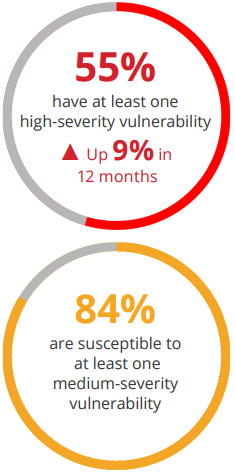
\includegraphics[width=\textwidth]{images/acunetix_vuln_report.png}
        \end{center}

        \column<2->{0.68\textwidth}
        \begin{itemize}

            \item
            Tipos de vulnerabilides incluidas\footnote[frame]{
                Acunetix Web Application Vulnerability Report 2016
                \textit{(Datos entre abril 2015 y marzo 2016)}
            }

            \begin{itemize}
                \item
                Severidad alta: XSS, Inyección SQL, entre otros

                \item
                Severidad media: CSRF, DoS, entre otros
            \end{itemize}
         \end{itemize}
    \end{columns}
\end{frame}

\begin{frame}
    \frametitle{Vulnerabilidades en aplicaciones web}

    \begin{itemize}[<+->]
        \item
        Estrategia de mitigación del riesgo de ataques:

        \begin{itemize}[<.->]
            \item
            Uso de Web Application Firewall (WAF)
        \end{itemize}
    \end{itemize}

    \begin{center}
        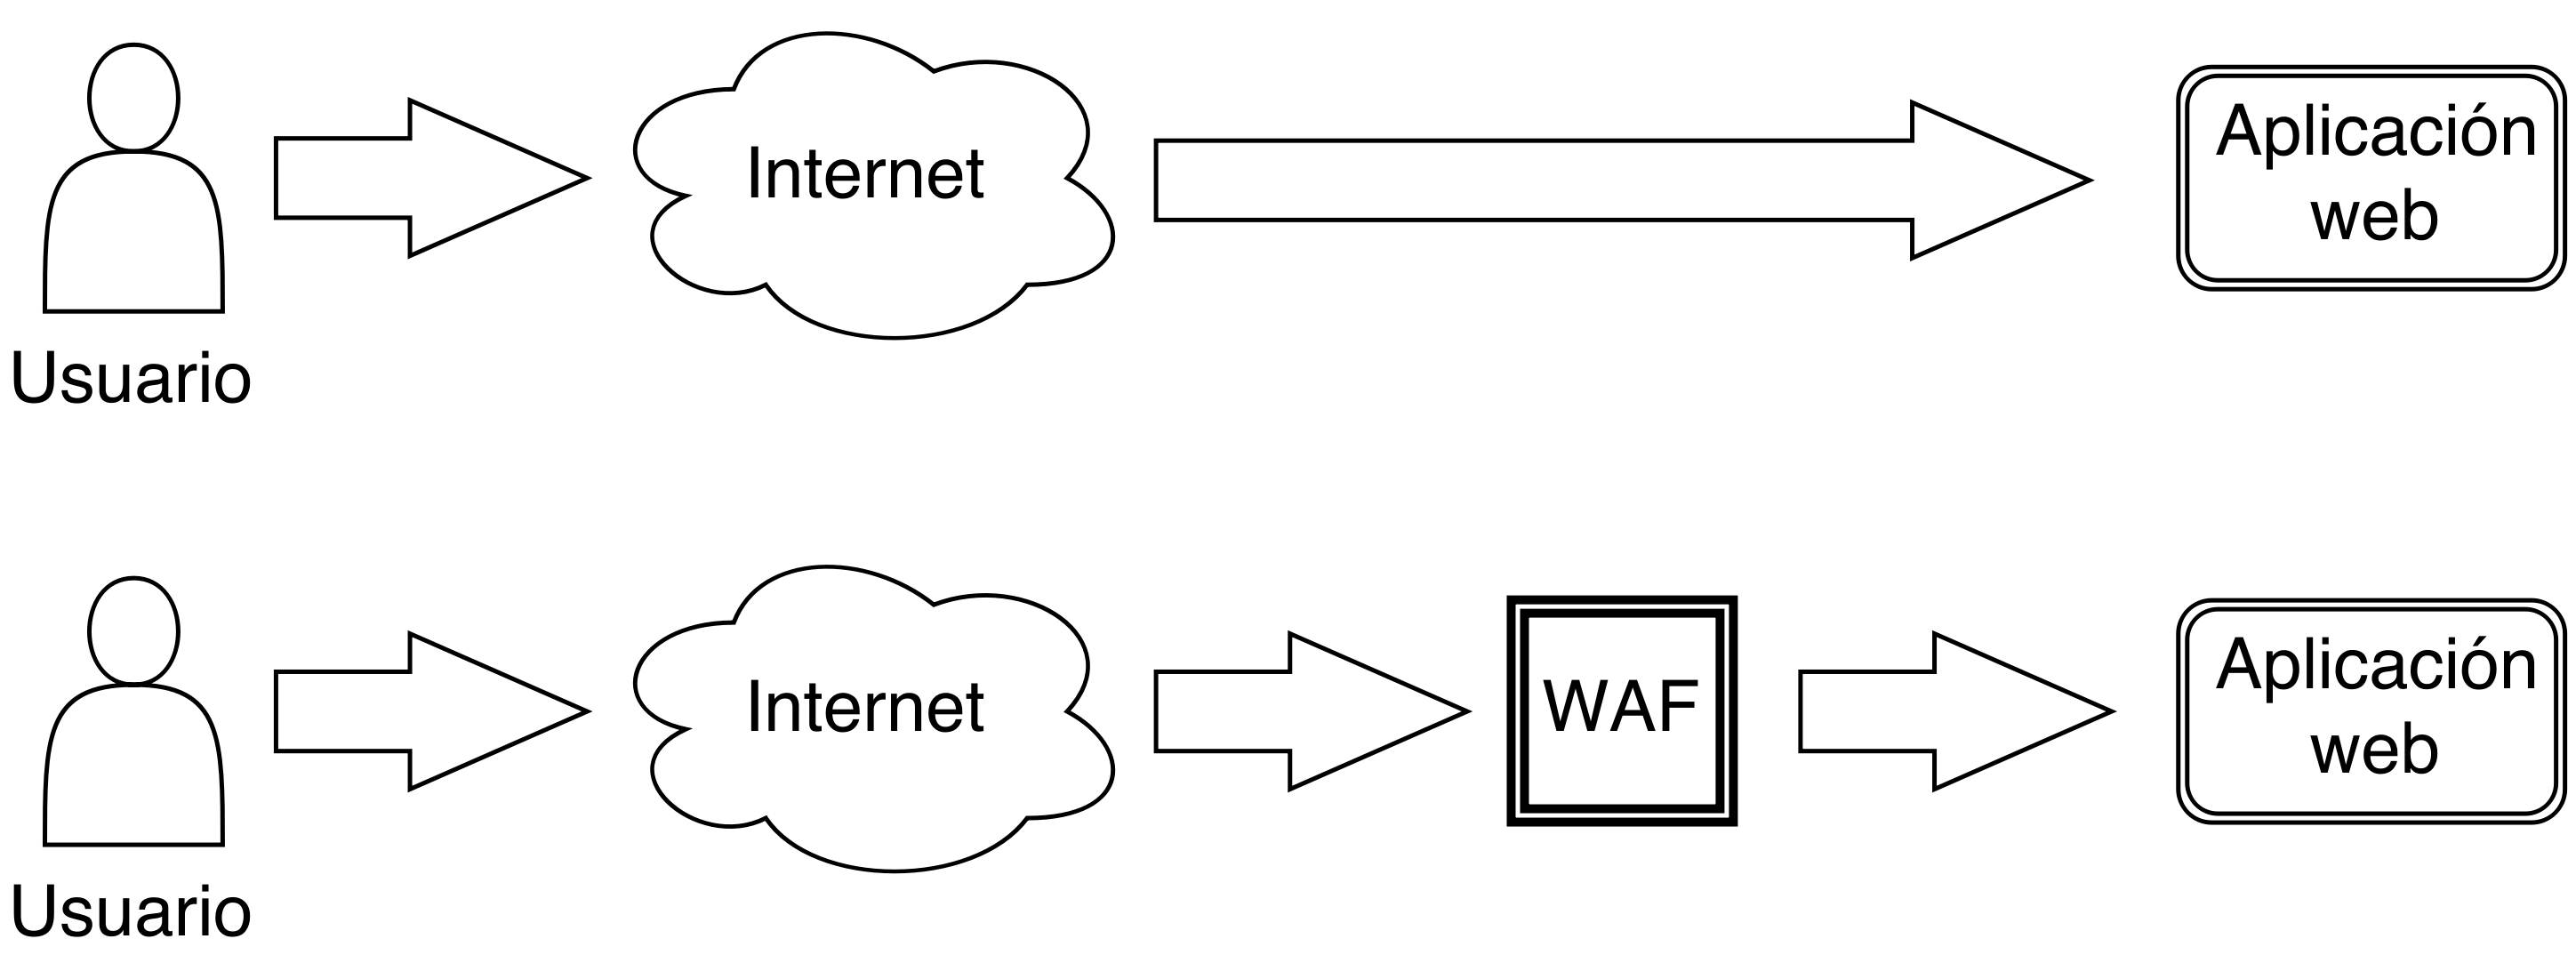
\includegraphics[width=\textwidth]{images/web-app.png}
    \end{center}
\end{frame}

\begin{frame}
    \begin{exampleblock}{Sistemas de Deteción de Intrusiones (IDS)}
        \begin{itemize}
            \item<2->
            Modo de respuesta:

            \begin{itemize}[<.->]
                \item
                Pasivo - detección (IDS)

                \item
                Activo - prevención (IPS)
            \end{itemize}

            \item<3->
            Fuente de datos:

            \begin{itemize}[<.->]
                \item
                \textit{Host-based systems} (HIDS)

                \item
                \textit{Network-based systems} (NIDS)

                \begin{itemize}
                    \item
                    Mensajes HTTP $\quad \rightarrow \quad$ WAF
                \end{itemize}
            \end{itemize}

            \item<4->
            Método de detección:

            \begin{itemize}[<.->]
                \item
                Por firmas de ataques

                \item
                Por anomalías
            \end{itemize}
        \end{itemize}
    \end{exampleblock}
\end{frame}

\begin{frame}
    \begin{exampleblock}{WAF con deteción de anomalías}
        \begin{itemize}
            \item<1->
            Dos fases:

            \begin{itemize}[<.->]
                \item
                Fase de entrenamiento: construcción de modelos que describen
                mensajes HTTP normales

                \item
                Fase de detección: comparación de nuevos mensajes con
                modelos construidos
            \end{itemize}

            \item<2->
            Ventaja: detección de ataques nuevos sin re-entrenar

            \item<2->
            Desventaja: dificultad de contrucción de modelos significativos

            \item<3->
            Estrategías de abordaje:

            \begin{itemize}[<.->]
                \item
                Métodos estadísticos (definición de \textit{threshold})

                \item
                Problema de clasificación utilizando herramientas de
                \textit{Machine Learning}
            \end{itemize}
        \end{itemize}
    \end{exampleblock}
\end{frame}

\begin{frame}
    \begin{exampleblock}{Problemas de clasificación y \textit{Machine Learning}}
        \begin{columns}
            \column{0.4\textwidth}
            \begin{center}
                \only<2>{
                    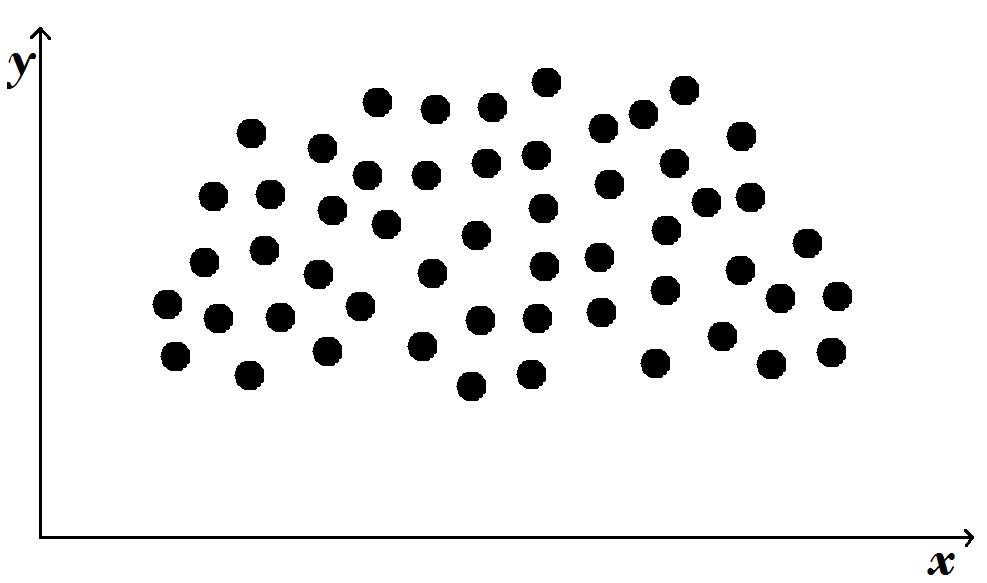
\includegraphics[width=\textwidth]{images/clasif-unsupervised.png}
                }
                \only<3>{
                    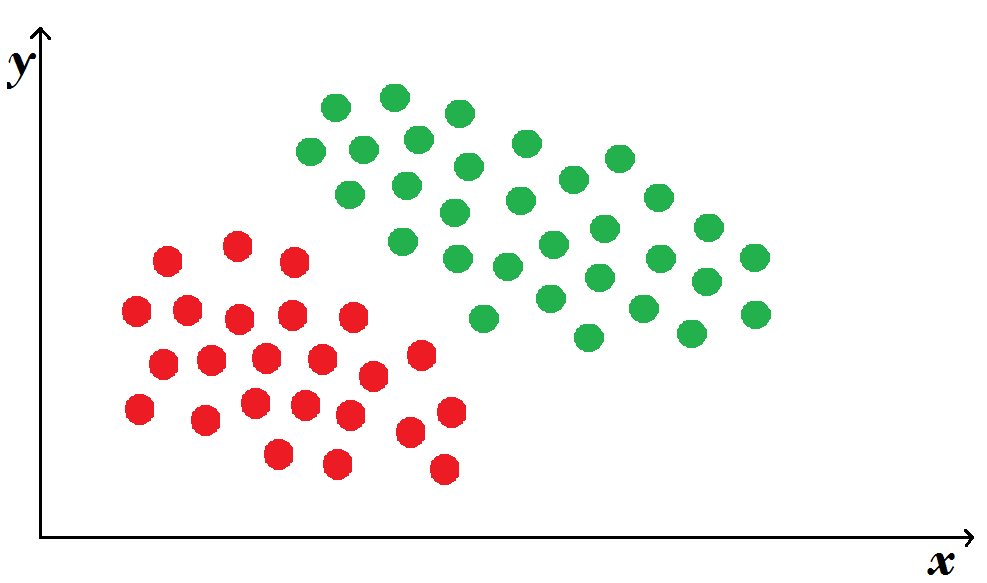
\includegraphics[width=\textwidth]{images/clasif-supervised.png}
                }
                \only<4>{
                    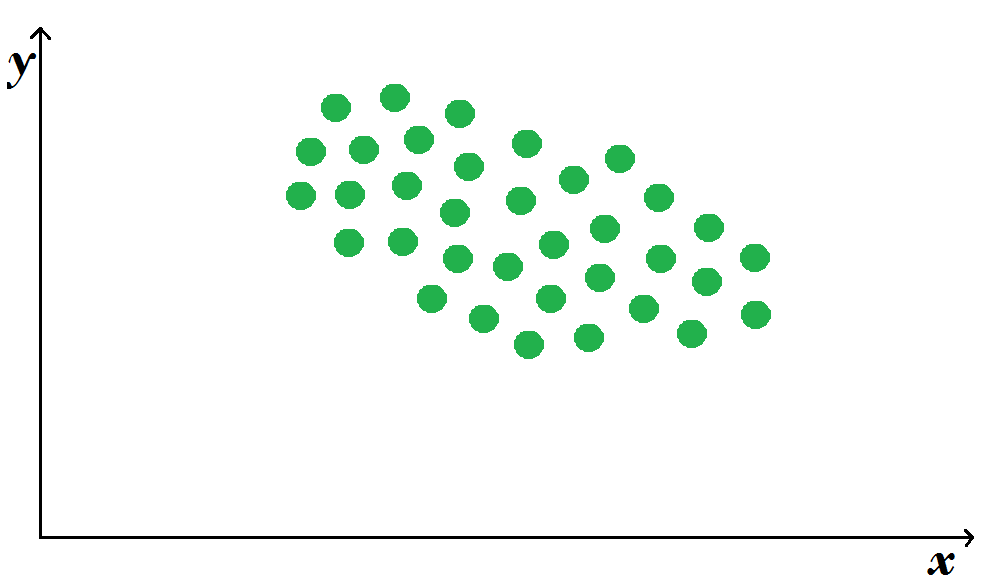
\includegraphics[width=\textwidth]{images/clasif-semi-supervised.png}
                }
            \end{center}

            \column{0.6\textwidth}
            \begin{itemize}[<+(1)->]
                \item
                Clasificación no supervisada

                \item
                Clasificación supervisada

                \item
                Clasificación semi-supervisada

                \begin{itemize}[<.->]
                    \item
                    Caso especial: entrenamiento con muestras de una sola clase
                    OCC: \textit{One-Class Classification}

                    \item
                    Una herramienta posible: One-Class SVM
                \end{itemize}
            \end{itemize}
        \end{columns}
    \end{exampleblock}
\end{frame}



\subsection{Objetivos para la investigación}

\begin{frame}
    \frametitle{Objetivo general}

    \begin{itemize}[<+(1)->]
        \item
        Detectar mensajes HTTP anómalos entre las aplicaciones web y
        sus usuarios con el fin de mitigar los riesgos de ataques contra
        dichas aplicaciones, utilizando un WAF basado en clasificadores
        One-Class SVM.
    \end{itemize}
\end{frame}

\begin{frame}
    \frametitle{Objetivos específicos}

    \begin{enumerate}[<+(1)->]
        \item
        Diseñar procesos de extracción de características (\textit{features})
        específicamente para mensajes HTTP, basado en aportes de otros
        investigadores de la literatura.

        \item
        Implementar un WAF basado en anomalías, utilizando los procesos de
        extracción de \textit{features} diseñados junto con clasificadores
        One-Class SVM.

        \item
        Evaluar la eficacia del WAF implementado en cuanto a la detección
        de mensajes HTTP anómalos.

        \item
        Analizar la viabilidad de utilizar el WAF implementado para
        detección de ataques en tiempo real.
    \end{enumerate}
\end{frame}

    \section{Implementación de OCS-WAF}



\subsection{Arquitectura general}

\begin{frame}
    \frametitle{Detector de anomalías OCS-WAF}

    \begin{center}
        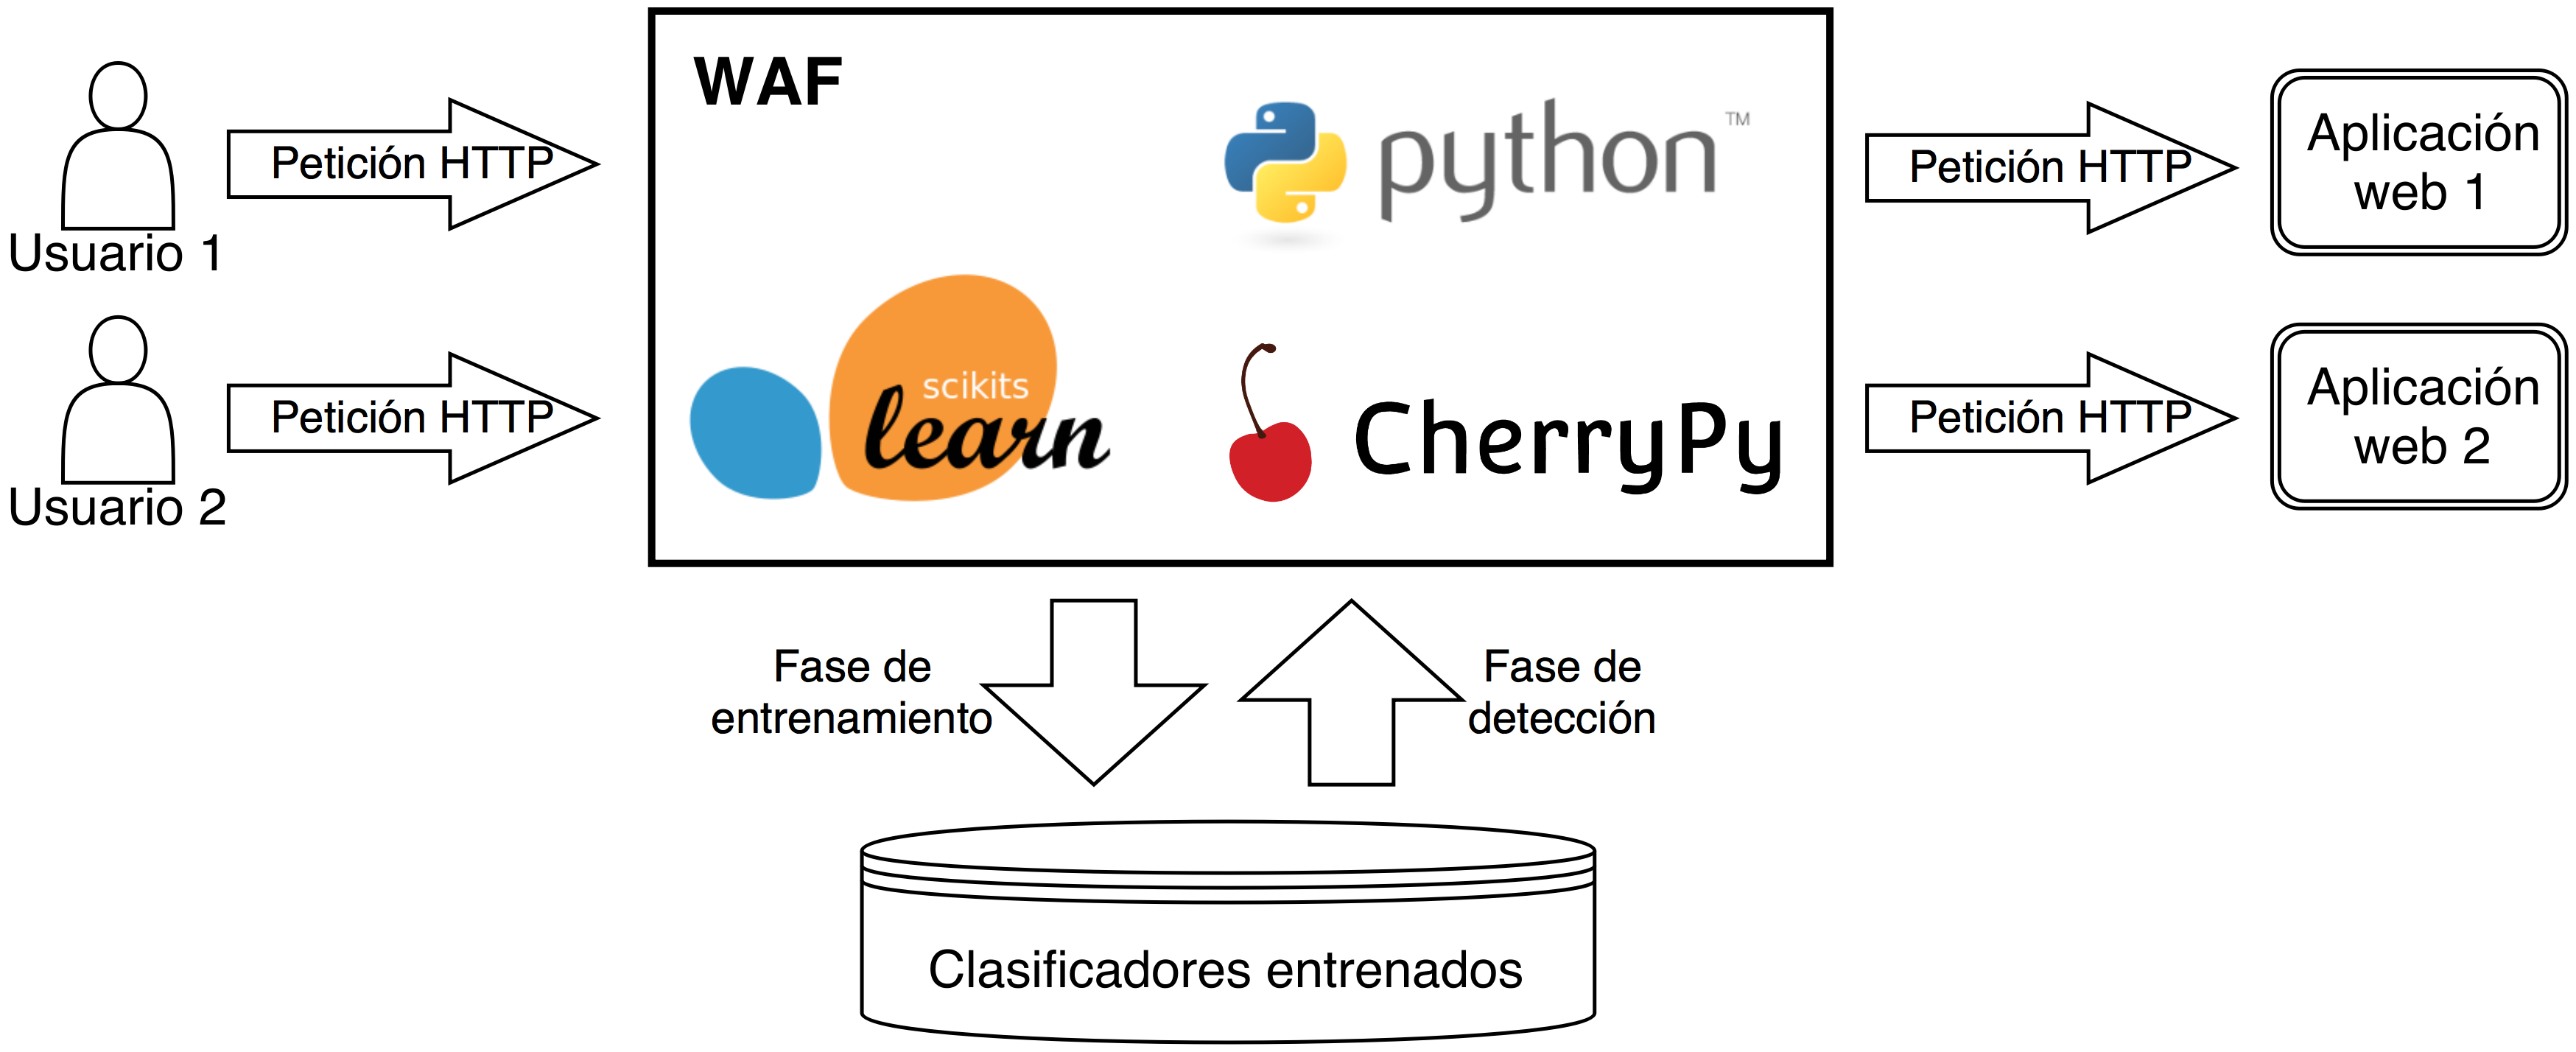
\includegraphics[width=\textwidth]{images/waf-diagram-overview.png}
    \end{center}

    \begin{flushleft}
        \begin{tabular}{l}
            
\includegraphics[height=0.5cm]{images/logo-github.jpg} \\
            \TheRepoUrl \\
        \end{tabular}
    \end{flushleft}
\end{frame}



\subsection{Fase de entrenamiento}

\begin{frame}
    \frametitle{Fase de entrenamiento de OCS-WAF}

    \begin{center}
        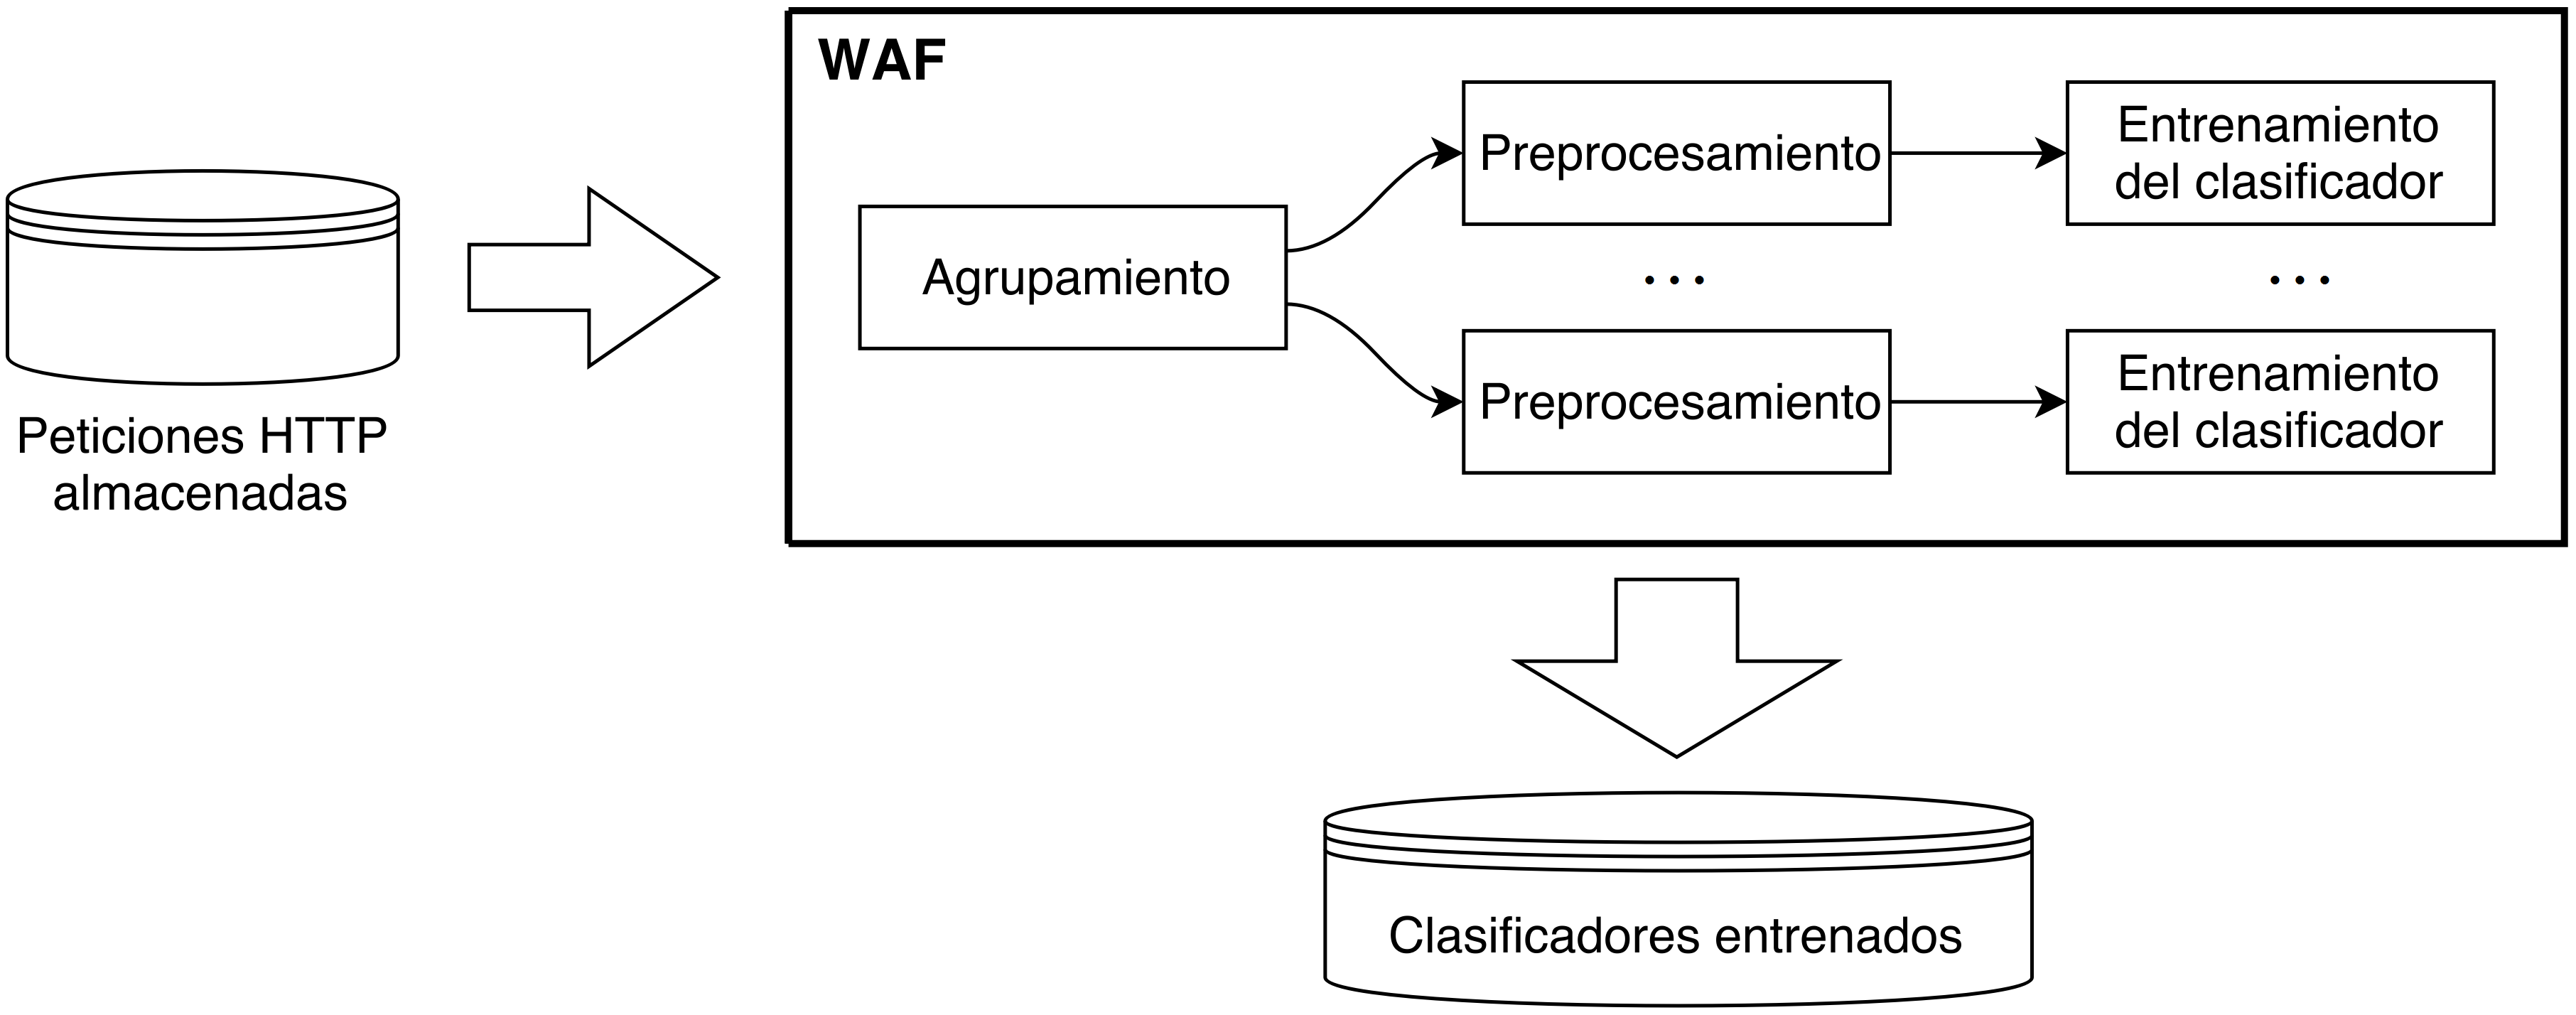
\includegraphics[width=\textwidth]{images/waf-diagram-training.png}
    \end{center}
\end{frame}

\begin{frame}
    \begin{exampleblock}{Estructura de peticiones HTTP}
        \begin{flushleft}
            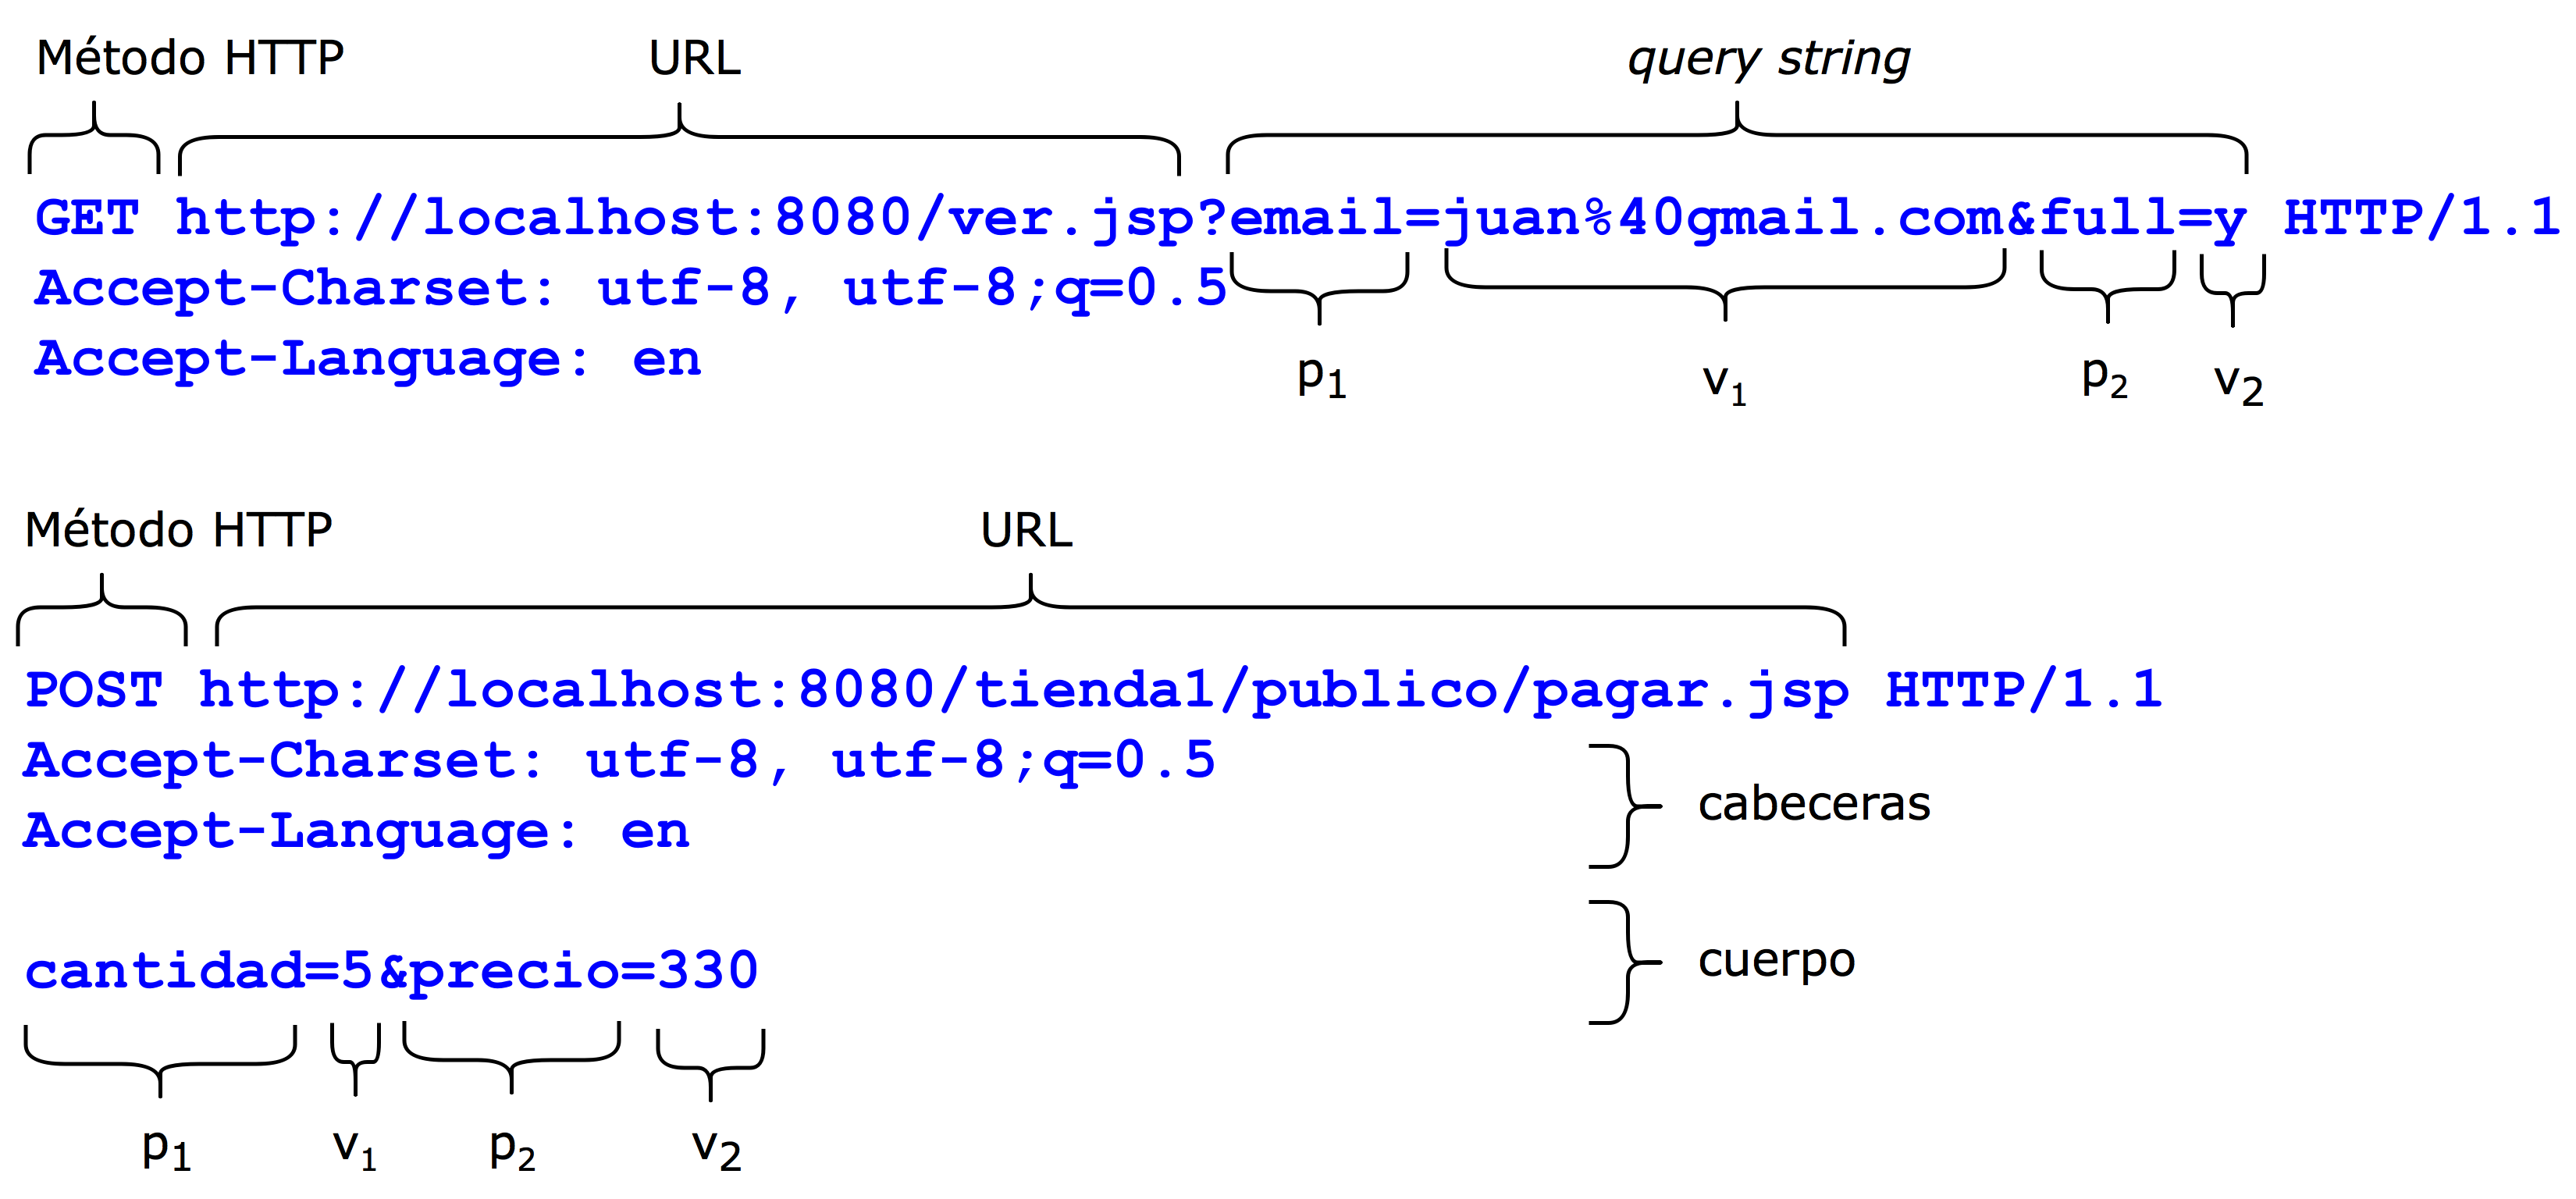
\includegraphics[width=\textwidth]{images/http-request-structure.png}
        \end{flushleft}
    \end{exampleblock}
\end{frame}

\begin{frame}
    \frametitle{1. Paso de agrupamiento}

    \begin{itemize}[<2->]
        \item
        Agrupación por método HTTP y URL

        \begin{flushleft}
            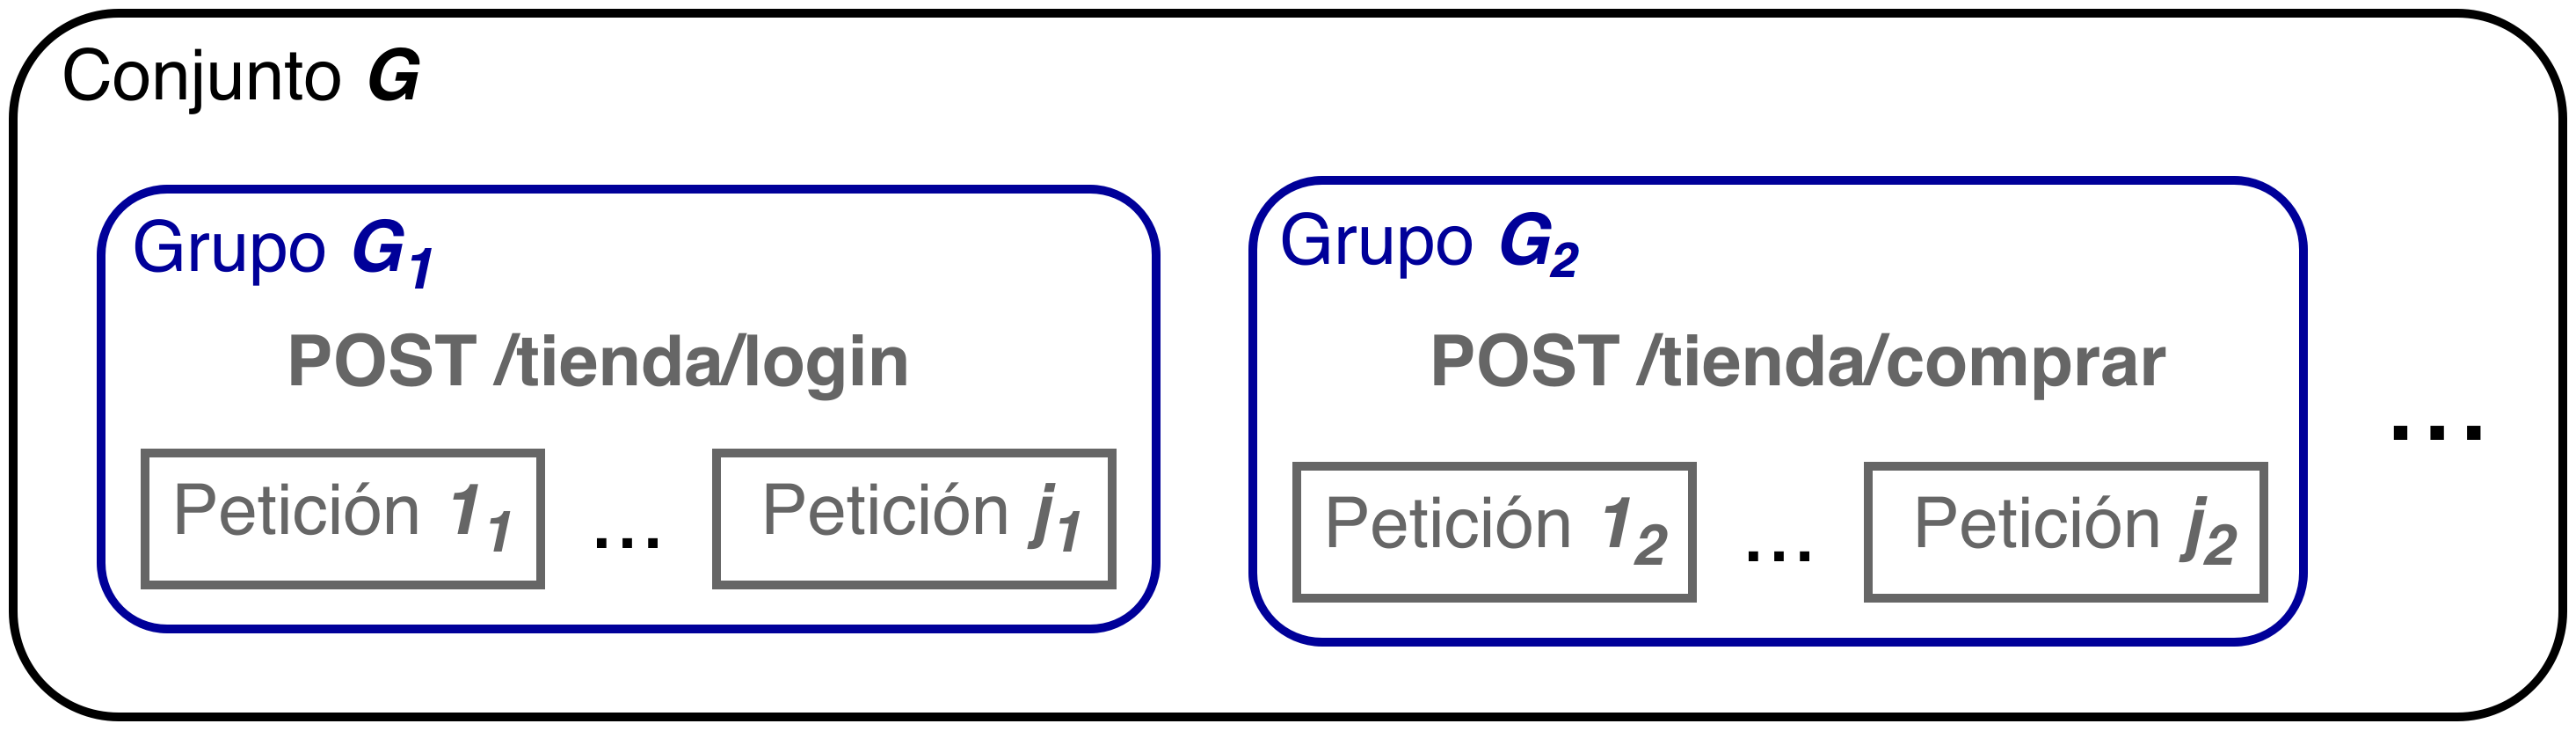
\includegraphics[width=0.9\textwidth]{images/request-groups.png}
        \end{flushleft}

        \item
        Similitud entre peticiones de un mismo grupo $G_{i}$

        \begin{itemize}[<.->]
            \item
            $ \forall i = 1, 2, \dots , \lvert G \rvert $
        \end{itemize}

        \item
        Descripciones más precisas del comportamiento normal dentro de
        cada grupo $G_{i}$
    \end{itemize}
\end{frame}

\begin{frame}
    \frametitle{2. Paso de preprocesamiento}

    \begin{itemize}[<+(1)->]
        \item
        Represetación de características de las peticiones mediante
        vectores numéricos de \textit{features}

        \begin{itemize}[<.->]
            \item
            Petición HTTP $ \quad \rightarrow \quad \vec{f} \in \mathbb{R}^{n} $

            \item
            dimensiones distintas para cada grupo $G_{i}$
        \end{itemize}

        \item
        Características analizadas por OCS-WAF:

        \begin{itemize}[<.->]
            \item
            Distribución de caracteres

            \item
            Entropía

            \item
            Cantidad de caracteres
        \end{itemize}
    \end{itemize}
\end{frame}

\begin{frame}[t]
    \frametitle{2. Paso de preprocesamiento}

    \begin{itemize}
        \item
        Distribución de caracteres

        \begin{itemize}
            \item
            Aporte de Kruegel y Vigna\footnote{
                Kruegel and Vigna (2003) \textit{Anomaly detection of
                web-based attacks}.}

            \item
            Distribución de frecuencias relativas de caracteres

            \item
            Suma de frecuencias relativas en cinco intervalos
        \end{itemize}
    \end{itemize}

    \only<2-3>{
        \begin{center}
            \begin{tikzpicture}
                \node (img1) {
                    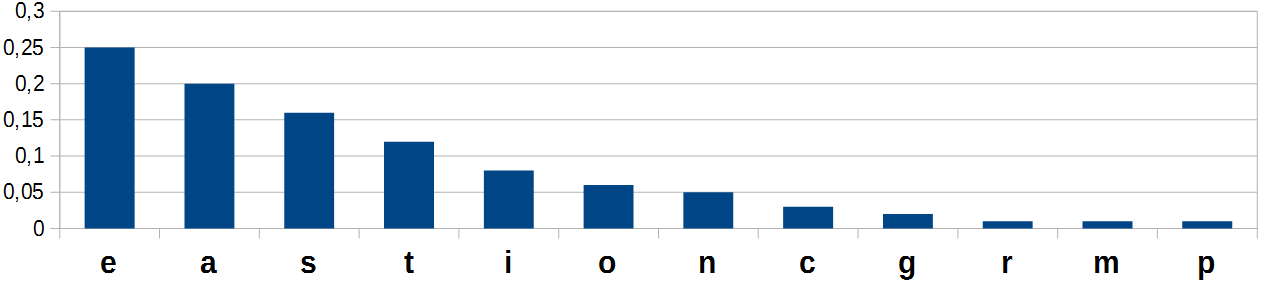
\includegraphics[width=\textwidth]{images/char-distr-blue1.png}
                };
                \node (img2) at (img1.south) [yshift=-0.1cm] {
                    
\includegraphics[width=\textwidth]{images/char-distr-intervals.png}
                };
                \node (img3) at (img1.north) [xshift=3.3cm,yshift=-0.8cm] {
                    \uncover<3->{
                        \frame{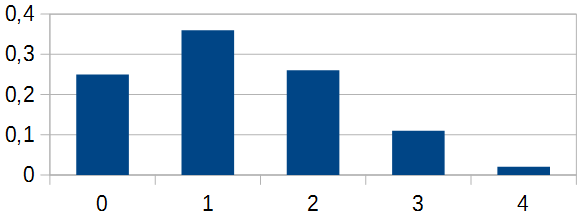
\includegraphics[width=0.4\textwidth]{images/char-distr-blue2.png}}
                    }
                };
            \end{tikzpicture}
        \end{center}
    }
    \only<4->{
        \begin{center}
            \begin{tikzpicture}
                \node (img1) {
                    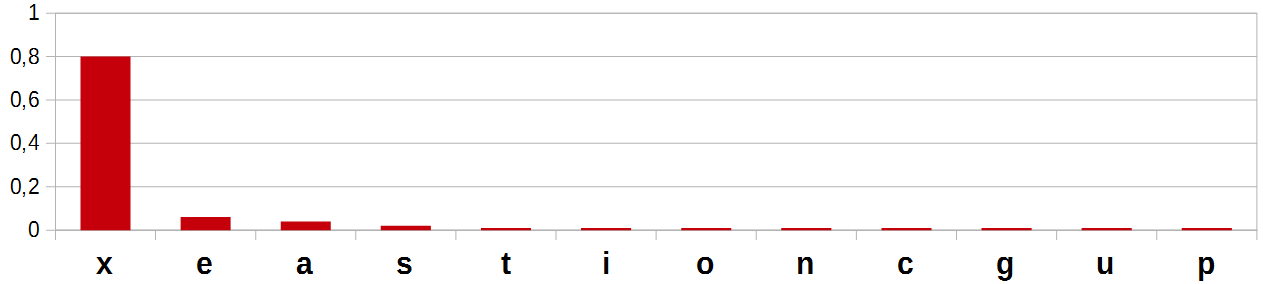
\includegraphics[width=\textwidth]{images/char-distr-red1.png}
                };
                \node (img2) at (img1.south) [yshift=-0.1cm] {
                    
\includegraphics[width=\textwidth]{images/char-distr-intervals.png}
                };
                \node (img3) at (img1.north) [xshift=3.3cm,yshift=-0.8cm] {
                    \uncover<5->{
                        \frame{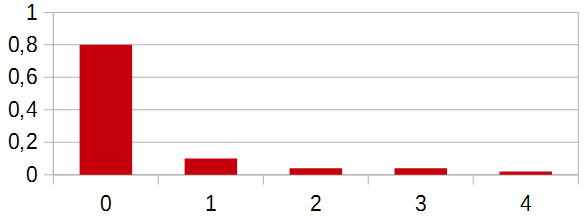
\includegraphics[width=0.4\textwidth]{images/char-distr-red2.png}}
                    }
                };
            \end{tikzpicture}
        \end{center}
    }
\end{frame}

\begin{frame}[t]
    \frametitle{2. Paso de preprocesamiento}

    \begin{itemize}
        \item
        Entropía (Teoría de la información)

        \begin{itemize}
            \item
            Relación entre longitud del valor y cantidad de caracteres
            distintos

            \item
            Aporte de Nguyen et. al.\footnote{
                Nguyen et. al. (2011) \textit{Application of the generic
                feature selection measure in detection of web attacks}.}

            \item
            Fórmula propuesta por Claude Shannon\footnote{
                Shannon (1948) \textit{A Mathematical Theory of Communication}.}
        \end{itemize}
    \end{itemize}

    \only<1>{
        \begin{columns}
            \column{0.6\textwidth}
            $$
            H(x) =
            - \sum_{i=1}^{\lvert c \rvert}
            \left(
                \frac{c_{i}}{\lvert x \rvert} \times \log_{2} \frac{c_{i}}{\lvert x \rvert}
            \right)
            $$

            \column{0.4\textwidth}
            \begin{block}{\small Ejemplo}
                \small
                $x = \text{aabbc}$

                $\lvert x \rvert = 5$

                $\lvert c \rvert = 3$

                $c_{1} = 2 \quad \rightarrow \quad \text{a}$

                $c_{2} = 2 \quad \rightarrow \quad \text{b}$

                $c_{3} = 1 \quad \rightarrow \quad \text{c}$
            \end{block}
        \end{columns}
    }
    \only<2->{
        \begin{columns}
            \column{0.4\textwidth}
            \begin{block}{\small Ejemplo: petición normal}
                \begin{itemize}
                    \item
                    \small $H(x) = \num{5.092}$
                \end{itemize}
            \end{block}

            \column{0.6\textwidth}
            \begin{block}{\small Ejemplo: petición con \textit{buffer overflow}}
                \begin{itemize}
                    \item
                    \small $H(x) = 0.901$
                \end{itemize}
            \end{block}
        \end{columns}
    }
\end{frame}

\begin{frame}[t]
    \frametitle{2. Paso de preprocesamiento}

    \begin{itemize}
        \item
        Cantidad de caracteres

        \begin{itemize}
            \item
            Aporte de Kruegel y Vigna\footnote{
                Kruegel and Vigna (2003) \textit{Anomaly detection of
                web-based attacks}.},
            y Nguyen et. al.\footnote{
                Nguyen et. al. (2011) \textit{Application of the generic
                feature selection measure in detection of web attacks}.}

            \item
            Conjuntos de caracteres

            \begin{enumerate}
                \item Todos
                \item Dígitos
                \item Letras
                \item Otros caracteres
            \end{enumerate}
        \end{itemize}
    \end{itemize}

    \uncover<2->{
        \begin{columns}
            \column{0.4\textwidth}
            \begin{block}{\small Ejemplo: petición normal}
                \vspace{-0.3cm}
                \begin{flushleft}
                    \small
                    \begin{tabular}{lcr}
                        Todos   & = & \num{100} \\
                        Dígitos & = &   \num{9} \\
                        Letras  & = &  \num{74} \\
                        Otros   & = &  \num{17} \\
                    \end{tabular}
                \end{flushleft}
            \end{block}

            \column{0.6\textwidth}
            \begin{block}{\small Ejemplo: petición con \textit{code injection}}
                \vspace{-0.3cm}
                \begin{flushleft}
                    \small
                    \begin{tabular}{lcr}
                        Todos   & = &       \num{132}  \\
                        Dígitos & = & \alert{\num{21}} \\
                        Letras  & = &        \num{78}  \\
                        Otros   & = & \alert{\num{33}} \\
                    \end{tabular}
                \end{flushleft}
            \end{block}
        \end{columns}
    }
\end{frame}

\begin{frame}
    \frametitle{2. Paso de preprocesamiento}

    \begin{itemize}
        \item
        10 \textit{features} extraídos
    \end{itemize}

    \begin{center}
        \small
        \begin{tabular}{|l|c|c|}
            \hline
            \multicolumn{1}{|c|}{\textit{Features}} & Tipo de dato & Rango de valores \\ \specialrule{1.5pt}{0}{0}
            Dist. de caract. - intervalo 0          & núm. reales  & $[0, 1]$         \\ \hline
            Dist. de caract. - intervalo 1          & núm. reales  & $[0, 1]$         \\ \hline
            Dist. de caract. - intervalo 2          & núm. reales  & $[0, 1]$         \\ \hline
            Dist. de caract. - intervalo 3          & núm. reales  & $[0, 1]$         \\ \hline
            Dist. de caract. - intervalo 4          & núm. reales  & $[0, 1]$         \\ \hline
            Entropía                                & núm. reales  & $[0, \infty)$    \\ \hline
            Longitud o cantidad total               & núm. enteros & $[0, \infty)$    \\ \hline
            Cantidad de dígitos                     & núm. enteros & $[0, \infty)$    \\ \hline
            Cantidad de letras                      & núm. enteros & $[0, \infty)$    \\ \hline
            Cantidad de otros caracteres            & núm. enteros & $[0, \infty)$    \\ \hline
        \end{tabular}
    \end{center}
\end{frame}

\begin{frame}
    \frametitle{2. Paso de preprocesamiento}

    \begin{itemize}[<+->]
        \item
        Análisis de valores de parámetros

        \begin{itemize}[<.->]
            \item
            Obtención de parámetros presentes en peticiones de $G_{i}$

            \begin{itemize}
                \item
                $ Q_{i} \ = \ [ \ \text{"email"} \ , \ \text{"full"} \ ] $

                \item
                $ B_{i} \ = \ [ \ ] $
            \end{itemize}

            \item
            Extracción de \textit{features} de cada valor de los parámetros
        \end{itemize}
    \end{itemize}

    \begin{flushleft}
        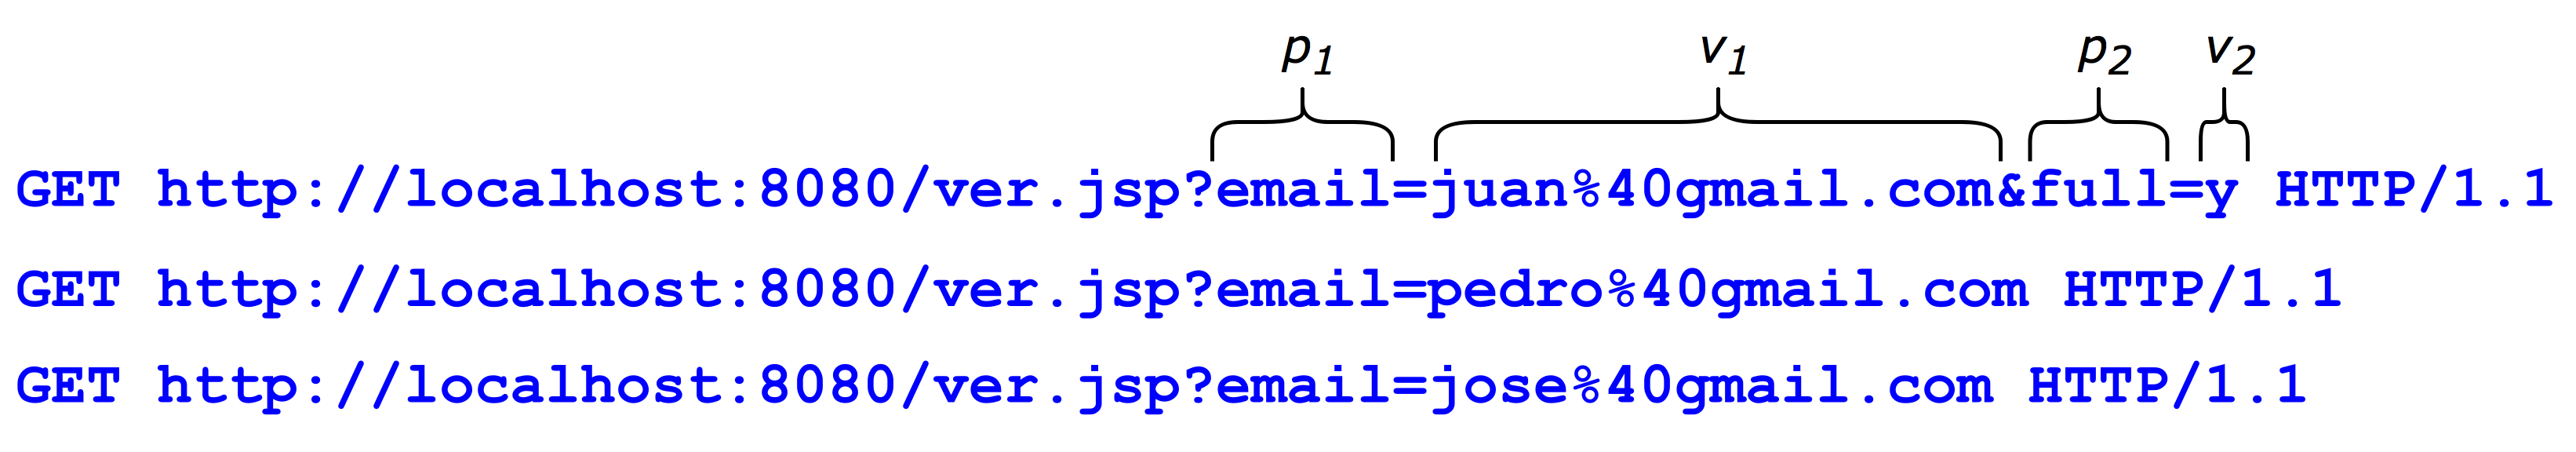
\includegraphics[width=\textwidth]{images/request-examples-1.png}
    \end{flushleft}
\end{frame}

\begin{frame}
    \frametitle{2. Paso de preprocesamiento}

    \begin{itemize}[<+->]
        \item
        Composición del vector de \textit{features}

        \begin{itemize}[<.->]
            \item
            Dimensiones según los parámetros en cada grupo $G_{i}$

            \item
            $ n_{i} = 10 \times \left( 1 + \lvert Q_{i} \rvert + \lvert B_{i} \rvert \right) $
        \end{itemize}
    \end{itemize}

    \begin{center}
        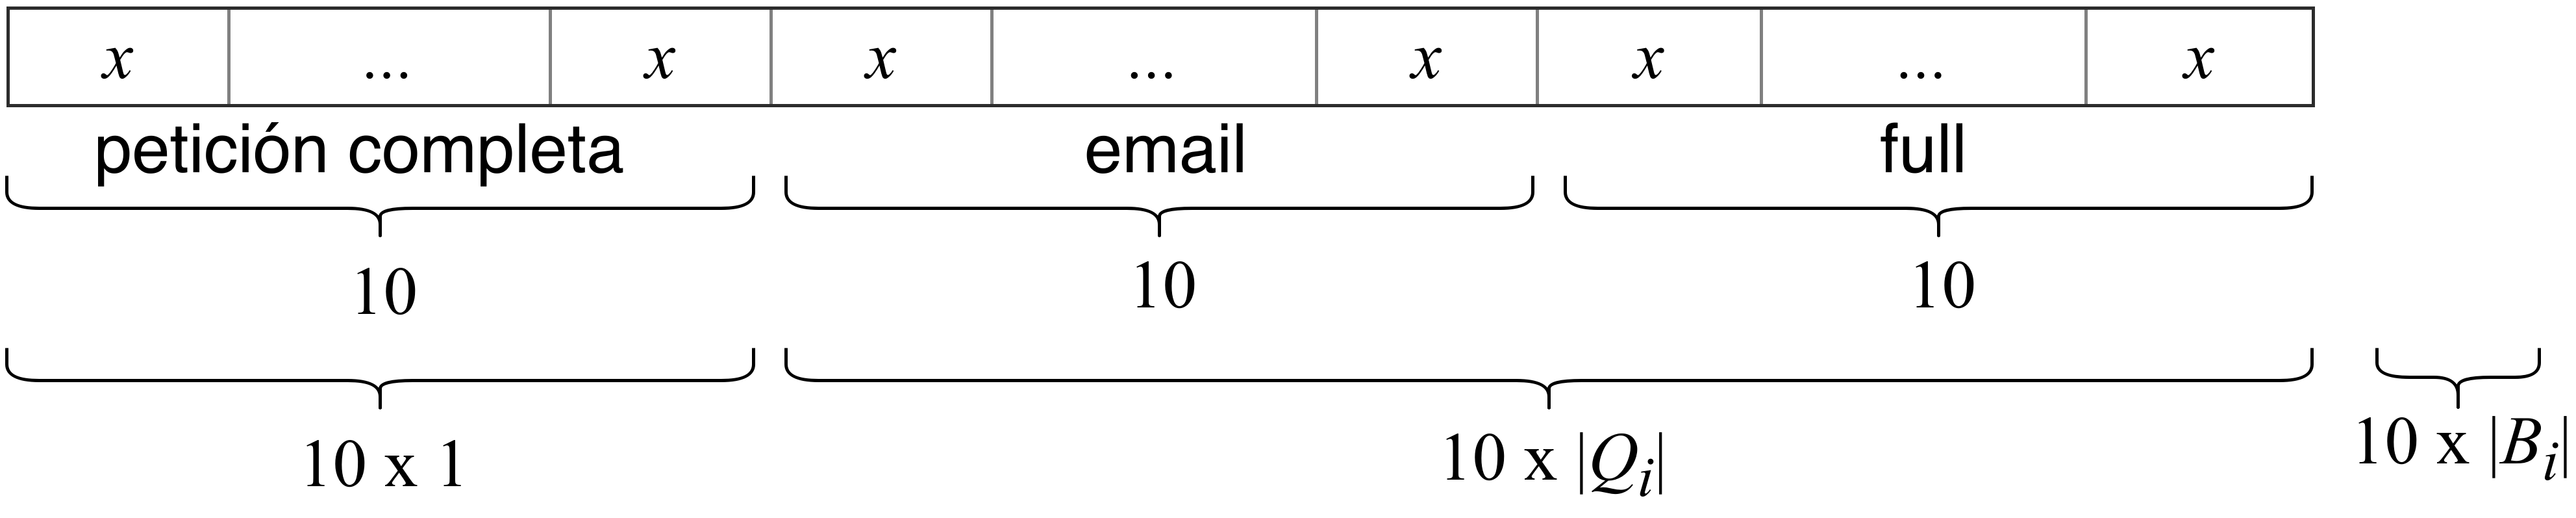
\includegraphics[width=\textwidth]{images/composition-vector.png}
    \end{center}

    \begin{flushleft}
        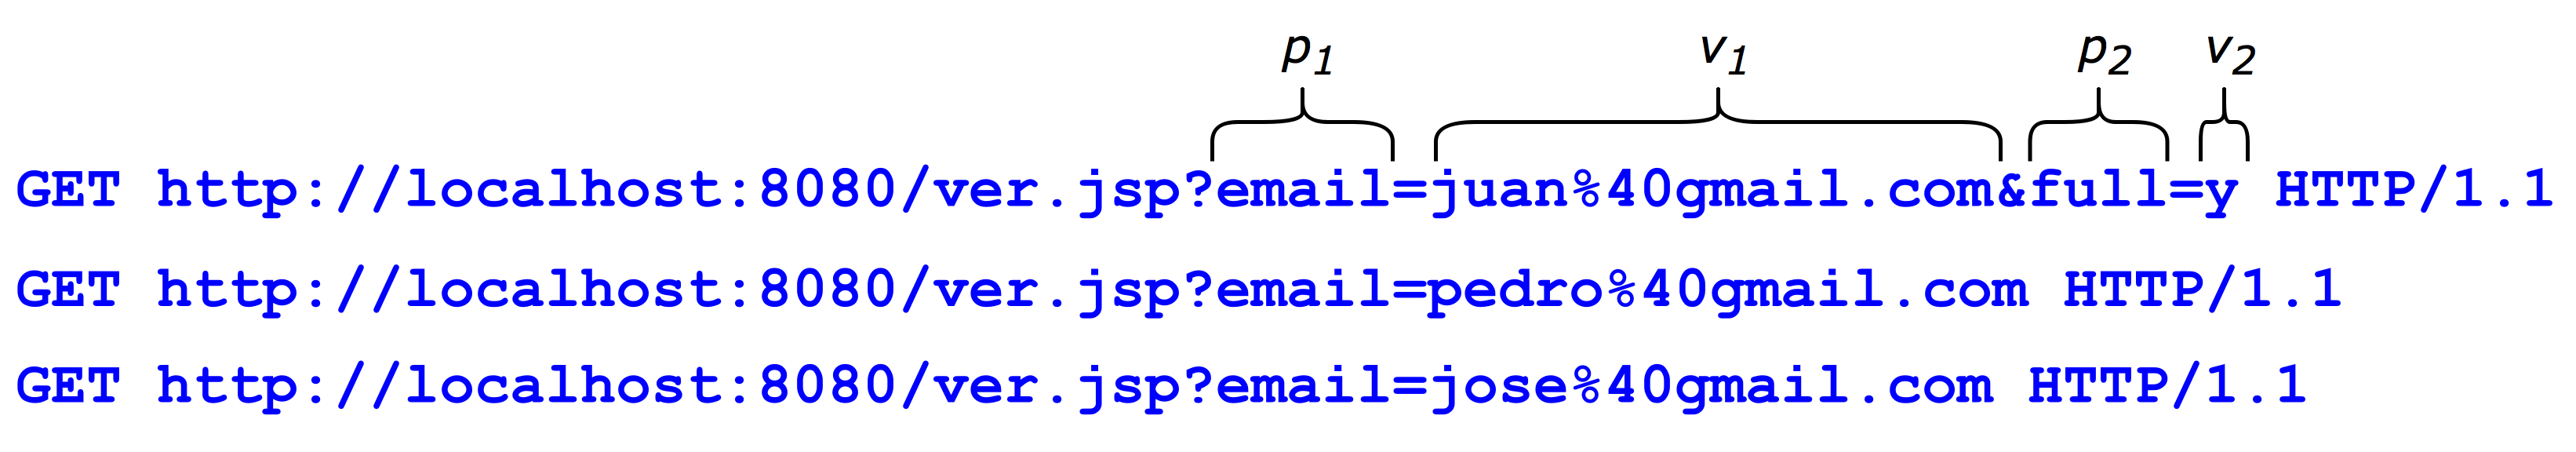
\includegraphics[width=\textwidth]{images/request-examples-1.png}
    \end{flushleft}
\end{frame}

\begin{frame}
    \frametitle{2. Paso de preprocesamiento}

    \begin{itemize}[<+->]
        \item
        Composición de la matriz de vectores de \textit{features}

        \begin{itemize}[<.->]
            \item
            Filas: vectores de peticiones del grupo $G_{i}$

            \item
            Columnas: \textit{features} del grupo $G_{i}$
        \end{itemize}
    \end{itemize}

    \begin{center}
        $$
        M_{i} =
        \begin{bmatrix}
            x_{1,1}                    & x_{1,2}                    & \cdots & x_{1,n_{i}} \\
            x_{2,1}                    & x_{2,2}                    & \cdots & x_{2,n_{i}} \\
            \vdots                     & \vdots                     & \ddots & \vdots      \\
            x_{\lvert G_{i} \rvert, 1} & x_{\lvert G_{i} \rvert, 2} & \cdots & x_{\lvert G_{i} \rvert, n_{i}}
        \end{bmatrix}
        $$
    \end{center}
\end{frame}

\begin{frame}
    \frametitle{2. Paso de preprocesamiento}

    \begin{itemize}
        \item
        Escalamiento de \textit{features} (normalización)

        \begin{itemize}
            \item
            Problema:

            \begin{itemize}
                \item
                Distintas importancias de \textit{features} debido a
                rangos diferentes
            \end{itemize}

            \item<2->
            Finalidad del escalamiento estándar\footnote{Rieck (2009) Machine
                Learning for Application-Layer Intrusion Detection}:

            \begin{itemize}[<2->]
                \item
                Promedio cercano a 0 y una varianza cercana a 1 en cada
                \textit{feature} (cada columna de $M_{i}$)
            \end{itemize}
        \end{itemize}
    \end{itemize}

    \uncover<2->{
        \begin{flushleft}
            $$
            x_{\text{\tiny nuevo}}
            \ = \
            \frac
                {x_{\text{\tiny actual}} - \mu_{\text{\tiny de la columna}}}
                {\sigma_{\text{\tiny de la columna}}}
            $$
        \end{flushleft}
    }
\end{frame}

\begin{frame}
    \begin{exampleblock}{\textit{Support Vector Machine} (SVM)}
        \begin{itemize}
            \item
            Clasificadores binarios de aprendizaje supervisado

            \item
            Separación de clases mediante un hiperplano
        \end{itemize}
    \end{exampleblock}

    \begin{columns}
        \column{0.5\textwidth}
        \uncover<2->{
            \begin{exampleblock}{One-Class SVM}
                \begin{itemize}
                    \item
                    Versión modificada para problemas OCC

                    \item
                    Separación de única clase del origen% mediante hiperplano

                    \item<3->
                    Transformación a otros espacios

                    \begin{itemize}[<.->]
                        \item
                        \textit{Radial Basis Function} (RBF) kernel
                    \end{itemize}
                \end{itemize}
            \end{exampleblock}
        }

        \column{0.5\textwidth}
        \begin{center}
            \only<1>{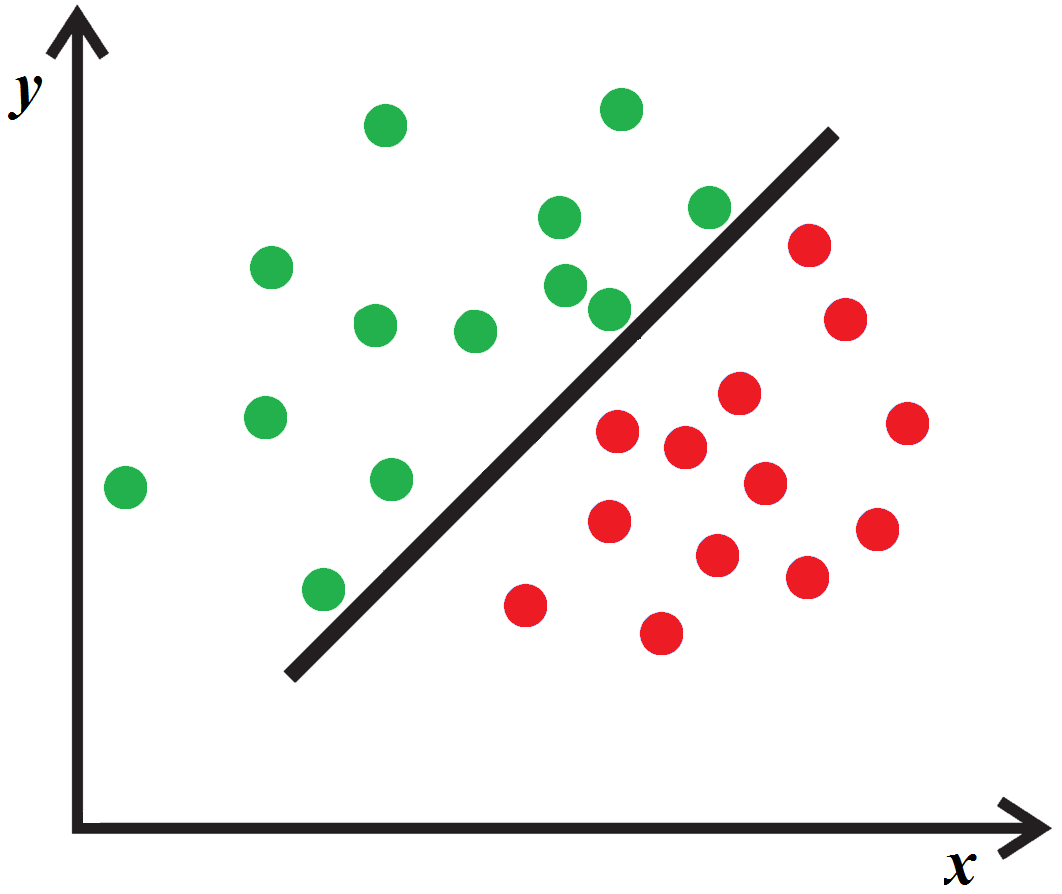
\includegraphics[width=\textwidth]{images/svm-example-1.png}}
            \only<2>{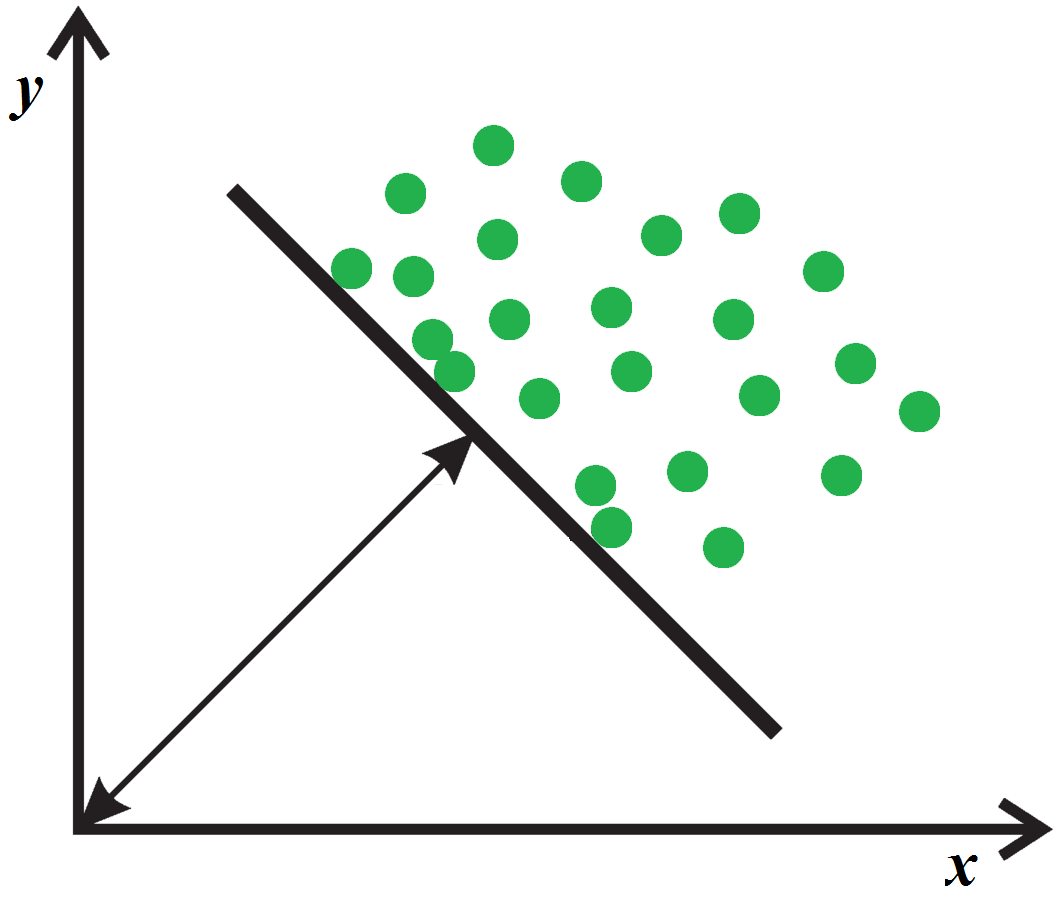
\includegraphics[width=\textwidth]{images/ocsvm-example-1.png}}
            \only<3->{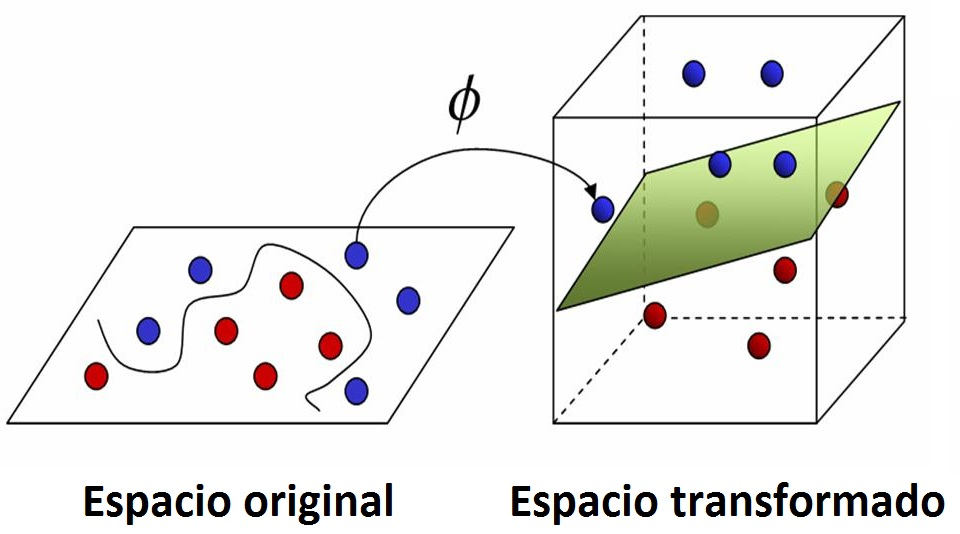
\includegraphics[width=\textwidth]{images/svm-transformed-space.jpg}}
        \end{center}
    \end{columns}
\end{frame}

\begin{frame}
    \frametitle{3. Paso de entrenamiento de clasificadores}

    \begin{columns}
        \column{0.5\textwidth}
        \begin{itemize}[<2->]
            \item
            Un One-Class SVM por cada grupo $G_{i}$

            \item
            Entrenamiento con los vectores de \textit{features}
            construidos

            \begin{itemize}[<.->]
                \item
                Matrices $M_{i}$
            \end{itemize}

            \item
            Gran cantidad de \textit{features}

            \item
            Almacenamiento persistente de clasificadores entrenados
        \end{itemize}

        \column{0.5\textwidth}
        \begin{center}
            \uncover<2->{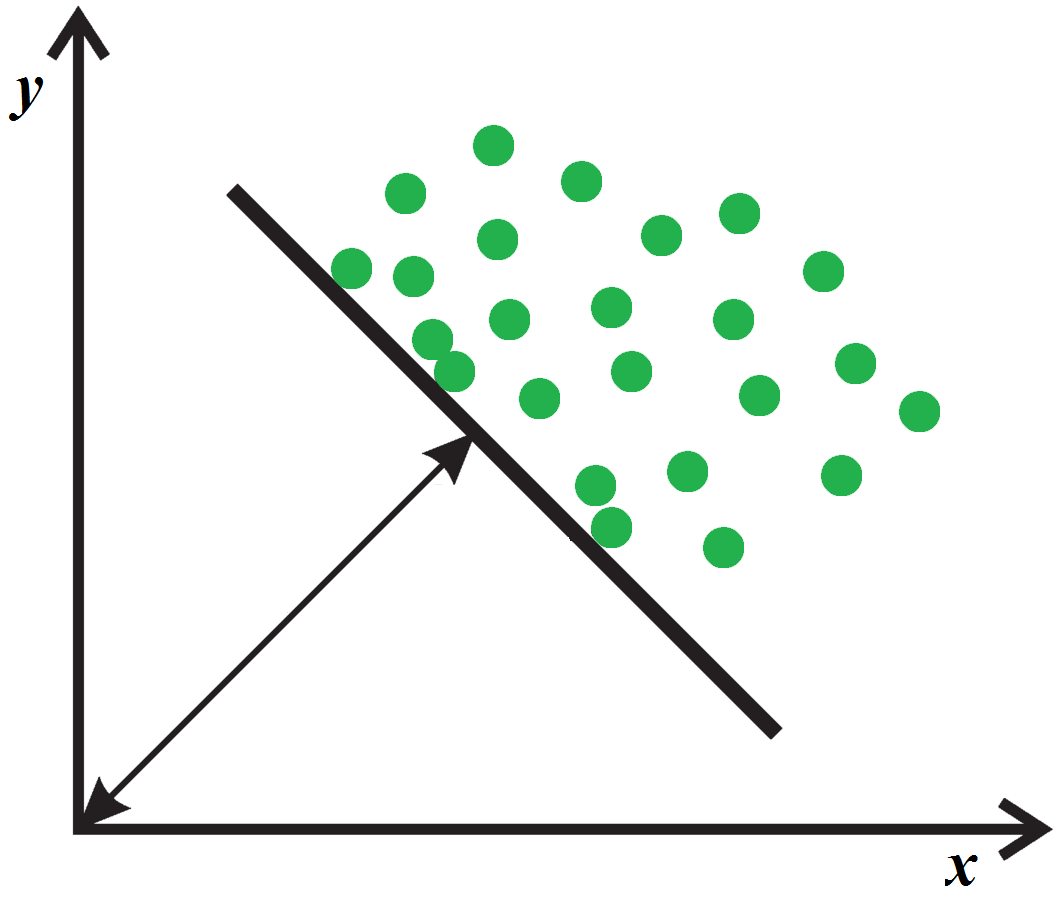
\includegraphics[width=\textwidth]{images/ocsvm-example-1.png}}
        \end{center}
    \end{columns}
\end{frame}



\subsection{Fase de detección}

\begin{frame}
    \frametitle{Fase de detección}

    \begin{center}
        \hspace*{-0.75cm}
        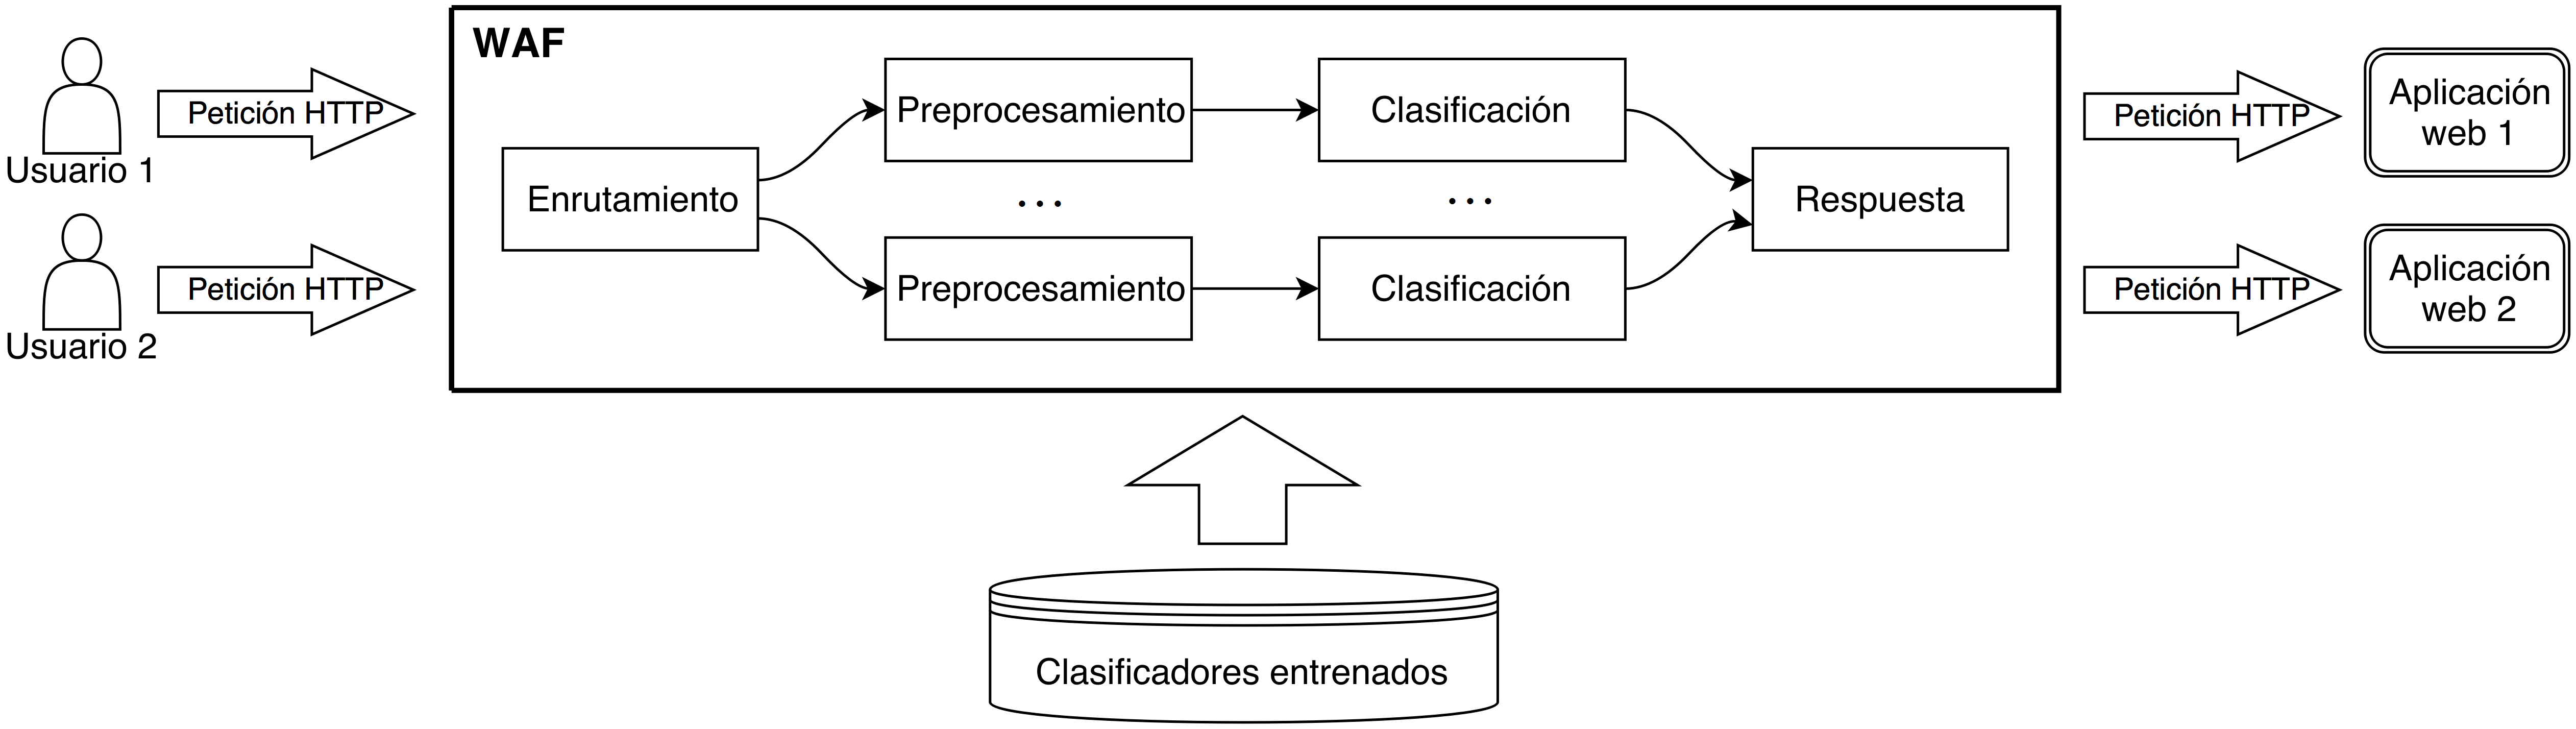
\includegraphics[width=1.1\textwidth]{images/waf-diagram-detection.png}
    \end{center}
\end{frame}

\begin{frame}
    \frametitle{1. Paso de enrutamiento}

    \begin{itemize}[<2->]
        \item
        Identificación del grupo $G_{i}$ de las nuevas peticiones según
        su método HTTP y URL

        \begin{flushleft}
            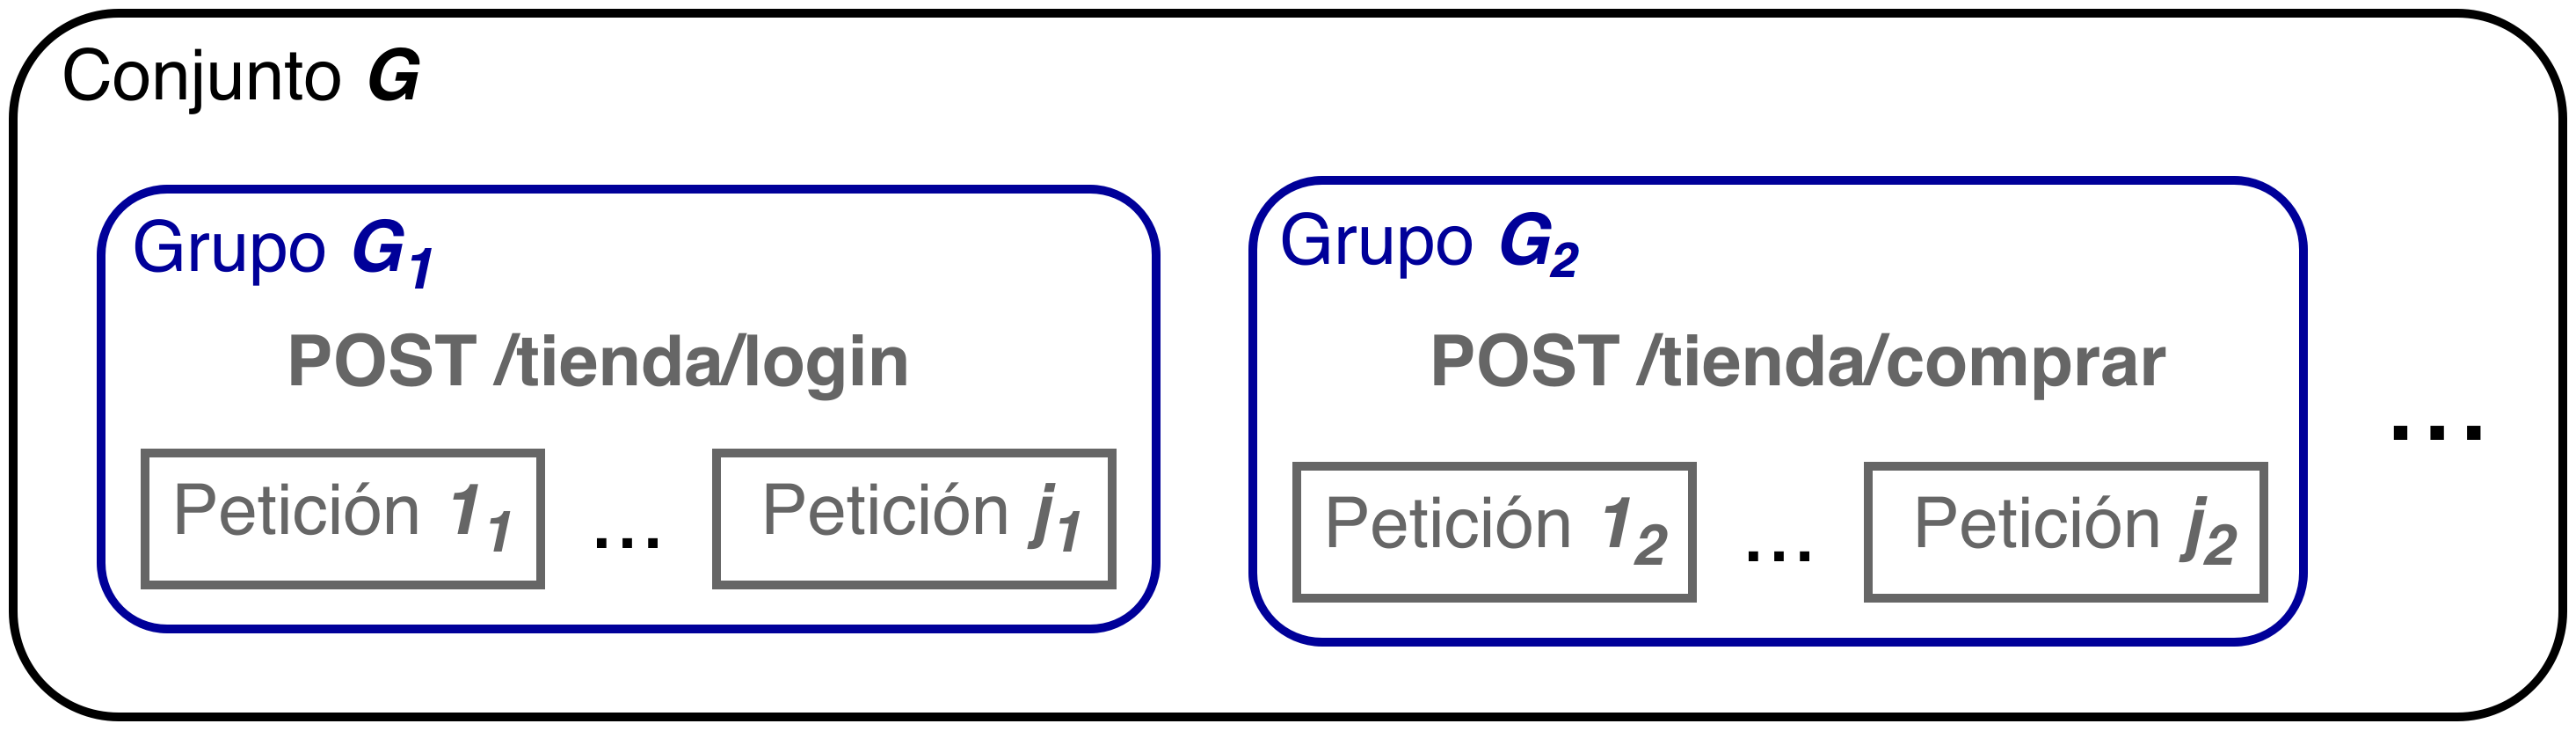
\includegraphics[width=0.9\textwidth]{images/request-groups.png}
        \end{flushleft}

        \item
        Delegación al proceso de extracción de \textit{features} del
        grupo y al clasificador correspondiente
    \end{itemize}
\end{frame}

\begin{frame}
    \frametitle{2. Paso de preprocesamiento}

    \begin{itemize}[<2->]
        \item
        Construcción de vectores de \textit{features} para nuevas peticiones

        \item
        Parámetro de $Q_{i}$ o $B_{i}$ que no aparece en una nueva petición

        \begin{itemize}[<.->]
            \item
            Componentes correspondientes llevan 0
        \end{itemize}

        \item
        Nuevos parámetros que no están en $Q_{i}$ o $B_{i}$

        \begin{itemize}[<.->]
            \item
            No agregan nuevos \textit{features} al vector

            \item
            Están contenidos en la petición completa
        \end{itemize}

        \item
        Vectores nuevos con misma dimensión $n_{i}$ del grupo
    \end{itemize}
\end{frame}

\begin{frame}
    \frametitle{3. Paso de clasificación}

    \begin{columns}
        \column{0.6\textwidth}
        \begin{itemize}[<2->]
            \item
            Uso del hiperplano obtenido para el grupo $G_{i}$

            \item
            Análisis de la posición de nuevas peticiones:

            \begin{itemize}
                \item
                Lado opuesto al origen:

                \begin{itemize}
                    \item
                    Petición normal
                \end{itemize}

                \item
                Mismo lado que el origen:

                \begin{itemize}
                    \item
                    Petición anómala o ataque
                \end{itemize}
            \end{itemize}
        \end{itemize}

        \column{0.4\textwidth}
        \begin{center}
            \uncover<2->{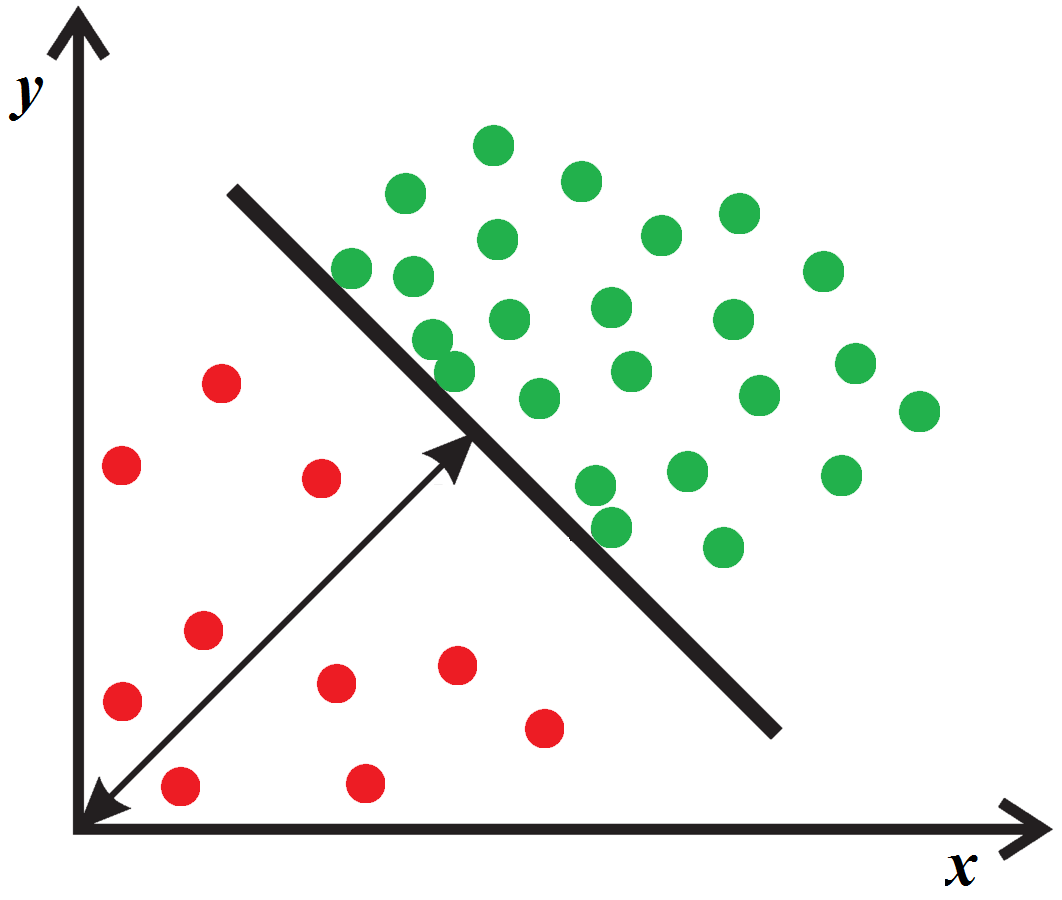
\includegraphics[width=\textwidth]{images/ocsvm-example-2.png}}
        \end{center}
    \end{columns}
\end{frame}

\begin{frame}
    \frametitle{4. Paso de respuesta}

    \begin{itemize}[<2->]
        \item
        Distintas acciones como respuesta al resultado de clasificación

        \item
        Peticiones normales:

        \begin{itemize}
            \item
            Reenvío a las aplicaciones web destino
        \end{itemize}

        \item
        Peticiones anómalas:

        \begin{itemize}
            \item
            Registro en un \textit{log}

            \item
            Opcionalmente: bloqueo de la petición
        \end{itemize}
    \end{itemize}
\end{frame}

    \section{Pruebas y resultados}



\subsection{Conjuntos de datos de prueba}

\begin{frame}
    \frametitle{Conjuntos de datos utilizados}

    \begin{itemize}
        \item
        Conjuntos utilizados:

        \begin{itemize}
            \item
            CSIC 2010\footnote{http://www.isi.csic.es/dataset/}

            \item
            CSIC TORPEDA 2012\footnote{http://www.tic.itefi.csic.es/torpeda}
        \end{itemize}

        \item
        Peticiones HTTP simuladas a una aplicación de comercio electrónico

        \item
        Distintos tipos de ataques

        \begin{itemize}
            \item
            Inyección SQL, \textit{buffer overflow}, \textit{cross-site scripting} (XSS),
            entre otros
        \end{itemize}

        \item
        Datos utilizados:

        \begin{itemize}
            \item
            18 grupos de peticiones según método HTTP y URL

            \item
            \num{40130} peticiones normales y \num{42444} anomalías
        \end{itemize}
    \end{itemize}
\end{frame}



\subsection{Análisis de la eficacia de detección}

\begin{frame}
    \frametitle{Pruebas de eficacia de detección}

    \begin{center}
        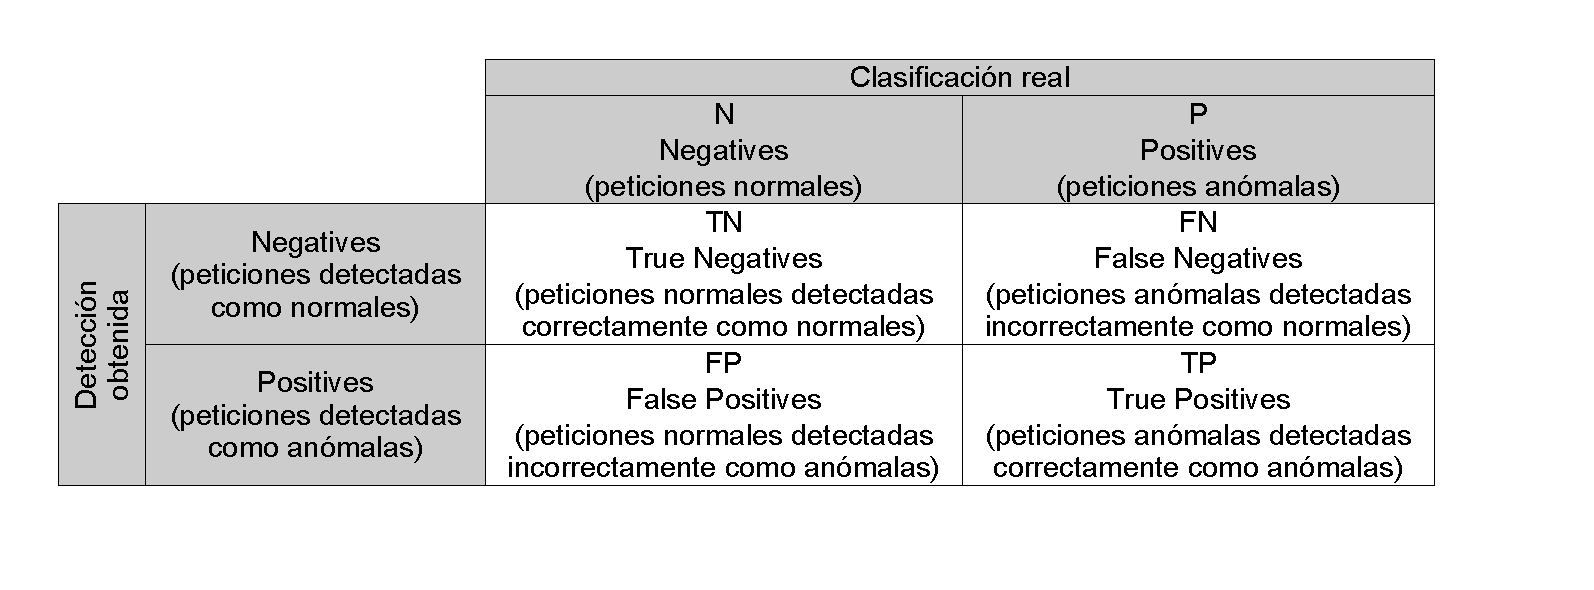
\includegraphics[width=\textwidth, trim=1.1cm 1.7cm 1.6cm 1cm]{images/diagram-score-explanation.pdf}
    \end{center}

    $$
    \text{TPR} = \frac{\text{TP}}{\text{P}}
    \quad , \ \quad
    \text{FPR} = \frac{\text{FP}}{\text{N}}
    \quad , \ \quad
    \text{F}_{1}\textit{-score} = \frac{2 \text{TP}}{2 \text{TP} + \text{FP} + \text{FN}}
    $$

    \begin{itemize}
        \item
        \small $\text{F}_{1}$-\textit{score} es más robusto frente a datos no balanceados
    \end{itemize}
\end{frame}

\begin{frame}
    \frametitle{Pruebas de eficacia de detección}

    \begin{itemize}
        \item
        Mejoras obtenidas por el análisis de valores de parámetros

        \begin{itemize}
            \item
            Promedio de los 18 grupos

            \item
            $\approx$ \num{2000} peticiones normales en cada grupo

            \item
            $\approx$ \num{1300} peticiones anómalas en cada grupo

            \item
            Usando \num{1500} peticiones para entrenamiento

            \begin{itemize}
                \item
                $\approx 75\%$ de los datos normales
            \end{itemize}

            \item
            3 iteraciones con distintos conjuntos de entrenamiento
        \end{itemize}
    \end{itemize}

    \begin{center}
        \small
        \begin{tabular}{|l|c|c|c|}
            \hline
                                       & TPR             & FPR             & F$_{1}$-\textit{score} \\ \specialrule{1.5pt}{0}{0}
            Solo petición completa     & $0.77 \pm 0.28$ & $0.11 \pm 0.22$ & $0.79 \pm 0.23$        \\ \hline
            Con análisis de parámetros & $0.93 \pm 0.11$ & $0.03 \pm 0.03$ & $0.95 \pm 0.08$        \\ \hline
        \end{tabular}
    \end{center}
\end{frame}



\subsection{Análisis del tiempo de respuesta de las aplicaciones}

\begin{frame}
    \frametitle{Pruebas de tiempo de respuesta}

    \begin{itemize}
        \item
        Medición del impacto de OCS-WAF sobre las aplicaciones protegidas

        \begin{itemize}
            \item
            Promedio de los 18 grupos

            \item
            100 peticiones de cada grupo
        \end{itemize}
    \end{itemize}

    \begin{center}
        \small
        \begin{tabular}{|l|r|}
            \hline
                                        & \multicolumn{1}{c|}{Tiempo de respuesta promedio} \\
                                        & \multicolumn{1}{c|}{(en milisegundos)}            \\
            \specialrule{1.5pt}{0}{0}
            Directo a la aplicación web & \num{4.0} $\pm$ \num{0.6}                         \\ \hline
            A través de OCS-WAF         & \num{8.7} $\pm$ \num{1.3}                         \\ \hline
        \end{tabular}
    \end{center}
\end{frame}



\subsection{Análisis del tiempo de entrenamiento}

\begin{frame}
    \frametitle{Pruebas de tiempo de entrenamiento}

    \begin{itemize}
        \item
        Medición de relación entre tiempo de entrenamiento y cantidad
        de peticiones utilizadas

        \begin{itemize}
            \item
            Duración máxima de los 18 grupos
        \end{itemize}
    \end{itemize}

    \begin{center}
        \small
        \begin{tabular}{|r|c|l|}
            \hline
            \multicolumn{1}{|c|}{Cantidad de} & Tiempo por petición & \multicolumn{1}{c|}{Duración} \\
            \multicolumn{1}{|c|}{peticiones}  & (en milisegundos)   & \multicolumn{1}{c|}{total}    \\
            \specialrule{1.5pt}{0}{0}
            \num{10}                          & \num{2.0}           & $< 1$ segundos                \\ \hline
            \num{100}                         & \num{1.7}           & $< 1$ segundos                \\ \hline
            \num{1000}                        & \num{1.7}           & $< 2$ segundos                \\ \hline
            \num{10000}                       & \num{1.8}           & $< 20$ segundos               \\ \hline
            \num{100000}                      & \num{7.0}           & $< 12$ minutos                \\ \hline
        \end{tabular}
    \end{center}
\end{frame}



\subsection{Compración con otros trabajos}

\begin{frame}
    \frametitle{Trabajos relacionados de otros autores}

    \begin{itemize}
        \item
        Utilización del mismo conjunto de datos CSIC 2010
    \end{itemize}

    \begin{center}
        \small
        \begin{tabular}{|l|c|c|c|}
            \hline
            \multicolumn{1}{|c|}{Sistema de detección} & TPR & FPR & F$_{1}$-\textit{score} \\
            \specialrule{1.5pt}{0}{0}
            OCS-WAF
            & \num{0.93} & \num{0.03} & \num{0.95} \\ \hline
            ModSecurity%
                \footnote{https://www.modsecurity.org/}
                \footnote{Giménez (2015) HTTP-WS-AD: Detector de
                    anomalías orientada a aplicaciones web y web services.}
            & \num{0.56} & \num{0.00} & \num{0.71} \\ \hline
            HTTP-WS-AD%
                \footnote{Giménez (2015) HTTP-WS-AD: Detector de
                    anomalías orientada a aplicaciones web y web services.}
            & \num{0.99} & \num{0.02} & \num{0.99} \\ \hline
            Árboles de decisión - Torrano-Giménez%
                \footnote{Torrano-Giménez (2015) Study of stochastic and
                    machine learning techniques for anomaly-based detection.}
            & \num{0.95} & \num{0.05} & -          \\ \hline
            OC-WAD%
                \footnote{Parhizkar y Abadi (2015) OC-WAD: A one-class
                    classifier ensemble approach for anomaly detection.}
            & \num{0.96} & \num{0.03} & -          \\ \hline
        \end{tabular}
    \end{center}
\end{frame}

    \section{Conclusiones}



\subsection{Resumen de la investigación}

\begin{frame}
    \frametitle{OCS-WAF}

    \begin{itemize}
        \item
        Implementación de un WAF para protección de múltiples aplicaciones
        web

        \item
        Detección de anomalías en mensajes HTTP mediante clasificadores
        One-Class SVM
    \end{itemize}

    \begin{center}
        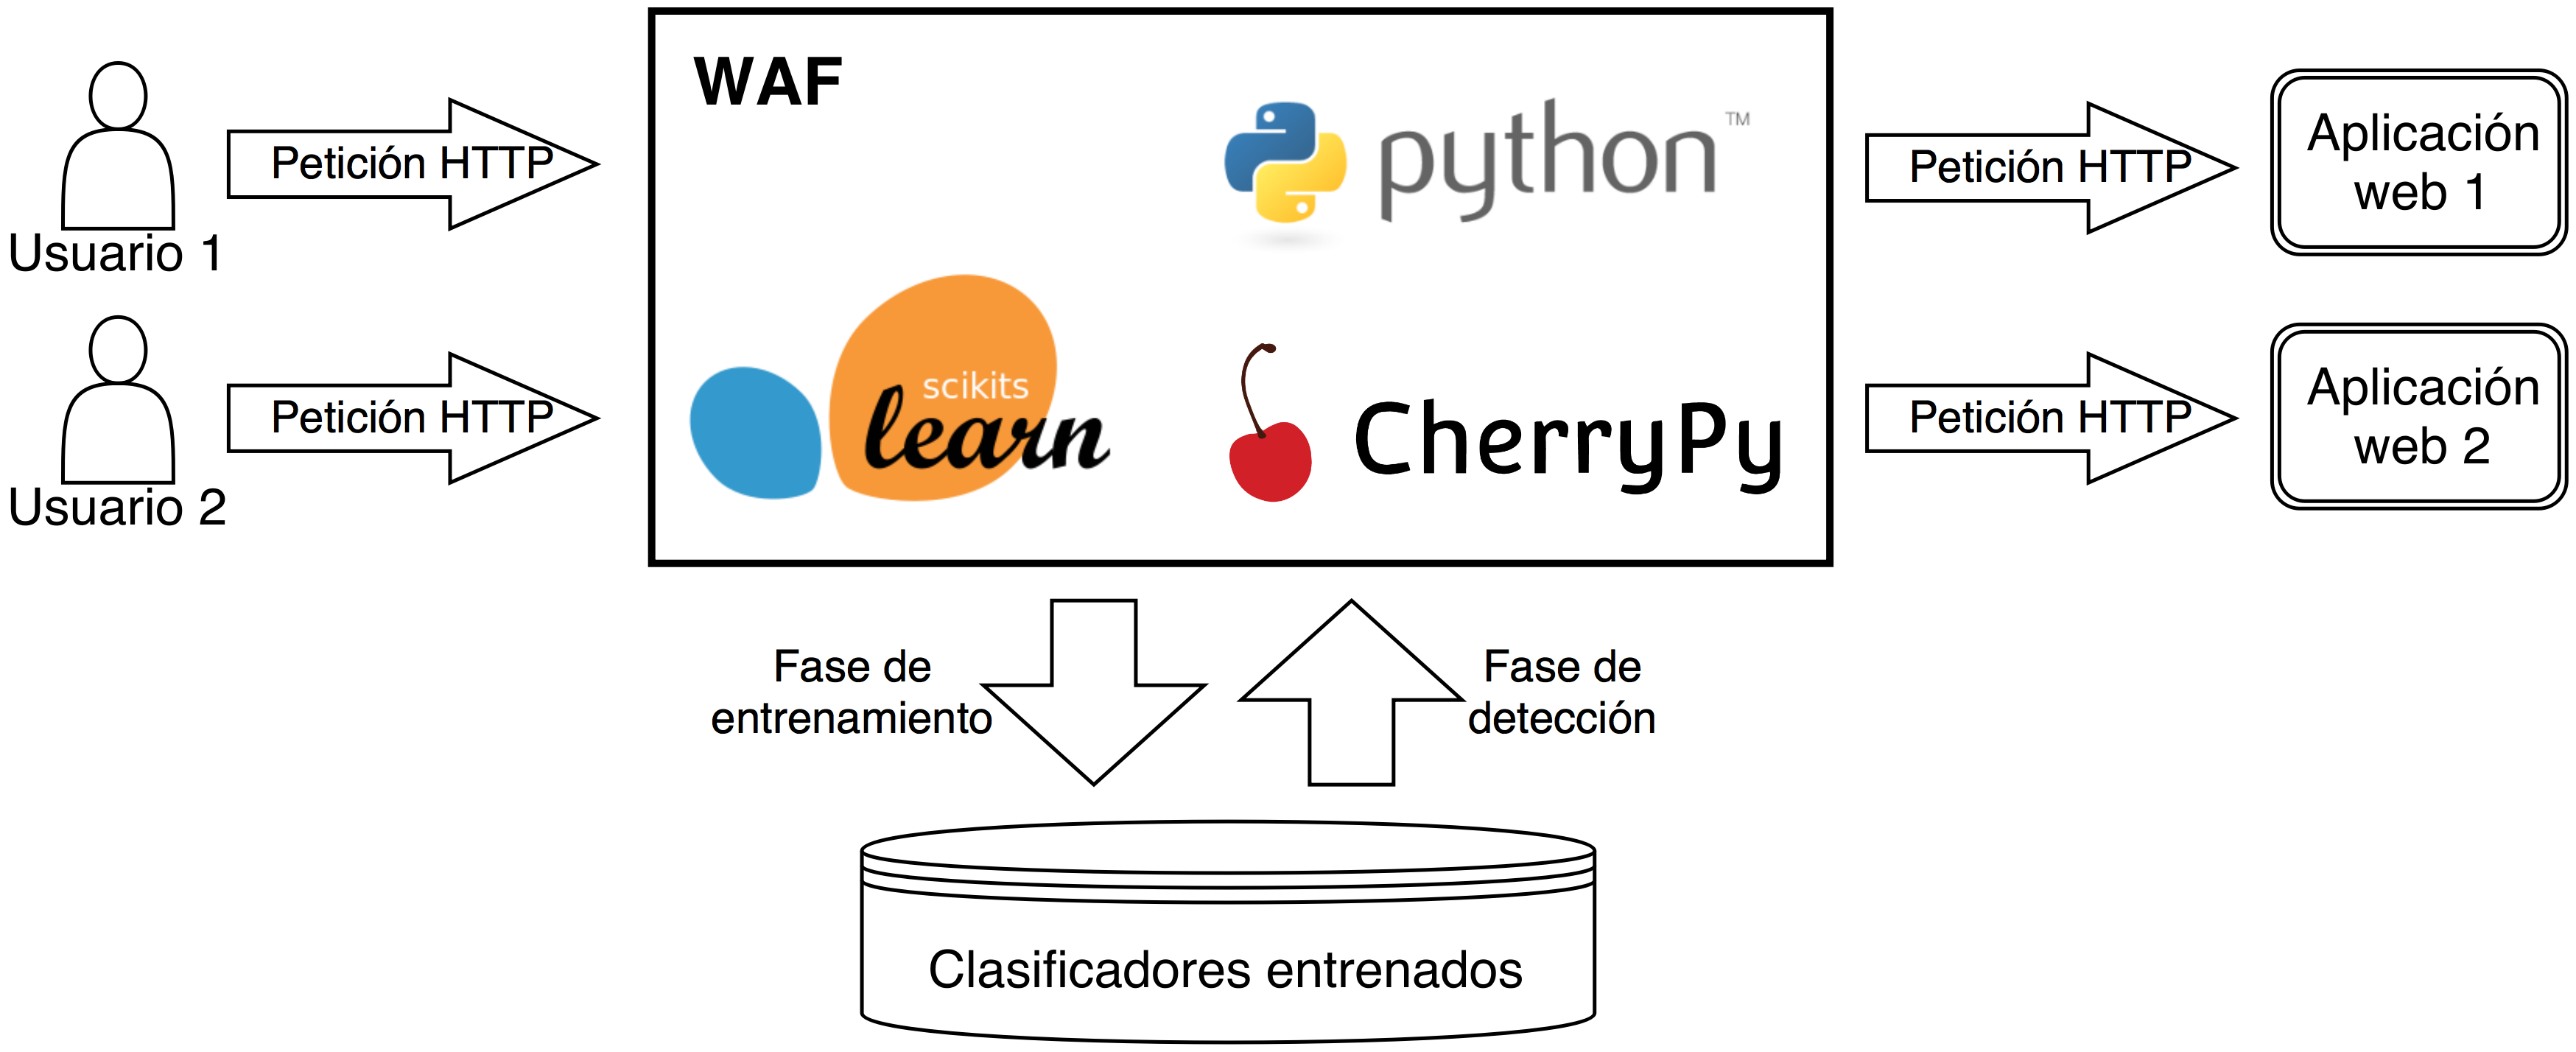
\includegraphics[width=\textwidth]{images/waf-diagram-overview.png}
    \end{center}
\end{frame}



\subsection{Logro de los objetivos}

\begin{frame}
    \frametitle{Objetivos específicos}

    \begin{enumerate}[<+(1)->]
        \item
        Diseñar procesos de extracción de características (\textit{features})
        específicamente para mensajes HTTP, basado en aportes de otros
        investigadores de la literatura.

        \begin{itemize}[<.->]
            \item
            Diseño de nuevos procesos de extracción de \textit{features}
            para mensajes HTTP
        \end{itemize}

        \item
        Implementar un WAF basado en anomalías, utilizando los procesos de
        extracción de \textit{features} diseñados junto con clasificadores
        One-Class SVM.

        \begin{itemize}[<.->]
            \item
            Implementación de OCS-WAF
        \end{itemize}

        \savemynewenumi
    \end{enumerate}
\end{frame}

\begin{frame}
    \frametitle{Objetivos específicos}

    \begin{enumerate}[<+->]
        \contmynewenumi

        \item
        Evaluar la eficacia del WAF implementado en cuanto a la detección
        de mensajes HTTP anómalos.

        \begin{itemize}[<.->]
            \item
            Pruebas de eficacia de detección con un
            TPR de \num{0.93},
            FPR de \num{0.03} y
            F$_{1}$-\textit{score} de \num{0.95}
        \end{itemize}

        \item
        Analizar la viabilidad de utilizar el WAF implementado para
        detección de ataques en tiempo real.

        \begin{itemize}[<.->]
            \item
            Realización de pruebas de impacto de OCS-WAF sobre el tiempo
            de respuesta de las aplicaciones protegidas
        \end{itemize}
    \end{enumerate}
\end{frame}

\begin{frame}
    \frametitle{Objetivo general}

    \begin{itemize}[<+(1)->]
        \item
        Detectar mensajes HTTP anómalos entre las aplicaciones web y
        sus usuarios con el fin de mitigar los riesgos de ataques contra
        dichas aplicaciones, utilizando un WAF basado en clasificadores
        One-Class SVM.

        \begin{itemize}[<.->]
            \item
            Detección de mensajes HTTP anómalos con OCS-WAF
        \end{itemize}
    \end{itemize}
\end{frame}



\subsection{Trabajos futuros}

\begin{frame}
    \frametitle{Ideas para trabajos futuros}

    \begin{itemize}[<+(1)->]
        \item
        Realizar pruebas con otros conjuntos de datos.

        \item
        Explorar otras características de los mensajes HTTP.

        \item
        Extender para incluir cuerpos de otros formatos, por ejemplo
        datos binario, JSON, XML, entre otros.

        \item
        Extender para incluir mensajes HTTP/2.

        \item
        Explorar la posibilidad de paralelizar el proceso de entrenamiento
        en OCS-WAF.
    \end{itemize}
\end{frame}



\subsection{Publicaciones}

\begin{frame}
    \frametitle{Publicación de nuestro trabajo}

    \begin{itemize}
        \footnotesize

        \item
        \textbf{Título:}
        Anomaly-based Web Application Firewall using HTTP-specific features
        and One-Class SVM
    \end{itemize}

    \begin{block}{\small WRSeg 2017}
        \begin{columns}
            \column{0.6\textwidth}
            \begin{itemize}
                \footnotesize

                \item
                Workshop Regional de Segurança da Informação e
                Sistemas Computacionais

                \item
                Santa María, Brasil

                \item
                25 de Setiembre 2017
            \end{itemize}

            \column{0.4\textwidth}
            \begin{center}
                
\includegraphics[width=\textwidth]{images/logo-errc2017.png}
            \end{center}
        \end{columns}
    \end{block}

    \begin{block}{\small Revista REABTIC}
        \begin{columns}
            \column{0.6\textwidth}
            \begin{itemize}
                \footnotesize

                \item
                Revista Eletrônica Argentina-Brasil de Tecnologias da Informação
                e da Comunicação

                \item
                Enviado para revisión
            \end{itemize}

            \column{0.4\textwidth}
            \begin{center}
                
\includegraphics[width=\textwidth]{images/logo-reabtic.png}
            \end{center}
        \end{columns}
    \end{block}
\end{frame}




    \section*{}     % the rest of the slides are not part of the outline

    \begin{frame}
        \begin{center}
            \LARGE
            Gracias por su atención!
        \end{center}

        \vfill

        \begin{center}
            \small
            \begin{tabular}{c}
                
\includegraphics[height=0.5cm]{images/logo-github.jpg} \\
                \TheRepoUrl \\
            \end{tabular}
        \end{center}
    \end{frame}

    \begin{frame}
    \frametitle{Anexo: One-Class SVM}

    \begin{itemize}
        \item
        \footnotesize Hiperplano del clasificador para el grupo $G_{i}$
    \end{itemize}

    \begin{equation}
        \vec{w_{i}} \cdot \phi(\vec{x})
        \ - \
        \rho_{i}
        \ = \
        \sum_{j=1}^{\lvert G_{i} \rvert}
        \left(
            a_{ij} \, K_{i}(\vec{f_{ij}}, \vec{x})
        \right)
        \ - \
        \rho_{i}
        \ = \
        0
    \end{equation}

    \begin{itemize}
        \item
        \footnotesize Kernel Radial Basis Function (RBF)
    \end{itemize}

    \begin{equation}
        K(\vec{x_{1}}, \vec{x_{2}})
        \ = \
        \phi(\vec{x_{1}}) \cdot \phi(\vec{x_{2}})
        \ = \
        \exp(
            - \gamma \lVert \vec{x_{1}} - \vec{x_{2}} \lVert^2
        )
    \end{equation}
\end{frame}

\begin{frame}
    \frametitle{Anexo: One-Class SVM}

    \begin{itemize}
        \item
        \footnotesize Entrenamiento: problema de minimización para el grupo $G_{i}$
    \end{itemize}

    \begin{equation}
        \min_{
            \vec{w_{i}}
            \ , \
            \rho_{i}
            \ , \
            \xi_{i}
        }
        \
        \frac{1}{2} \lVert {\vec{w_{i}}} \rVert^2
        \ - \
        \rho_{i}
        \ + \
        \frac{1}{\nu_{i} \lvert G_{i} \rvert} \sum_{j=1}^{\lvert G_{i} \rvert} \xi_{ij}
    \end{equation}

    \begin{equation}
        \vec{w_{i}} \cdot \phi(\vec{f_{ij}}) \geqslant \rho_{i} - \xi_{ij}
        \ , \quad
        \xi_{ij} \geqslant 0
        \ , \quad
        \forall j = 1,2, \dots, \lvert G_{i} \rvert
    \end{equation}

    \begin{itemize}
        \item
        \footnotesize Entrenamiento: formulación dual de la optimización
    \end{itemize}

    \begin{equation}
        \min_{a_{i}}
        \
        \frac{1}{2} \ a_{i} \ S_{i} \ a_{i}^{T}
    \end{equation}

    \begin{equation}
        \sum_{j=1}^{\lvert G_{i} \rvert} a_{ij} \ = \ 1
        \ , \quad
        0 \leqslant a_{ij} \leqslant \frac{1}{\nu_{i} \lvert G_{i} \rvert}
        \
        \forall j = 1,2, \dots, \lvert G_{i} \rvert
    \end{equation}
\end{frame}

\begin{frame}
    \frametitle{Anexo: One-Class SVM}

    \begin{itemize}
        \item
        \footnotesize Detección: función de decisión del grupo $G_{i}$
    \end{itemize}

    \begin{equation}
        g_{i}(\vec{x})
        \ = \
        \begin{cases}
            \vec{w_{i}} \cdot \phi(\vec{x}) - \rho_{i} \ \geqslant \ 0  & +1 \\
            \text{caso contrario}                                       & -1
        \end{cases}
    \end{equation}

    \begin{equation}
        g_{i}(\vec{x})
        \ = \
        \begin{cases}
            \sum_{j=1}^{\lvert G_{i} \rvert}
            \left(
                a_{ij} \, K_{i}(\vec{f_{ij}}, \vec{x})
            \right)
            - \rho_{i} \ \geqslant \ 0  & +1 \\
            \text{caso contrario}       & -1
        \end{cases}
    \end{equation}
\end{frame}

\begin{frame}
    \frametitle{Anexo: Datos utilizados para las pruebas}

    \begin{itemize}
        \item
        \footnotesize Información sobre los 18 grupos de peticiones
    \end{itemize}

    \begin{center}
        \tiny
        \begin{tabularx}{\linewidth}{|C|c|ll|r|r|r|}
            \hline
            ID
            & \multicolumn{1}{c|}{\begin{tabular}[c]{@{}c@{}}Conjunto\\ de datos\\ CSIC\end{tabular}}
            & \multicolumn{2}{c|}{Método HTTP y URL}
            & \multicolumn{1}{c|}{\begin{tabular}[c]{@{}c@{}}Cant.\\ parám.\end{tabular}}
            & \multicolumn{1}{c|}{\begin{tabular}[c]{@{}c@{}}Peticiones\\ normales\end{tabular}}
            & \multicolumn{1}{c|}{\begin{tabular}[c]{@{}c@{}}Peticiones\\ anómalas\end{tabular}} \\
            \specialrule{1.5pt}{0}{0}
            c00 & 2010  & GET  & /tienda1/miembros/editar.jsp         & 13 &  \num{2000} &  \num{1362} \\ \hline
            c01 & 2010  & POST & /tienda1/miembros/editar.jsp         & 13 &  \num{2000} &  \num{1362} \\ \hline
            c02 & 2010  & GET  & /tienda1/publico/anadir.jsp          &  5 &  \num{2000} &  \num{1380} \\ \hline
            c03 & 2010  & POST & /tienda1/publico/anadir.jsp          &  5 &  \num{2000} &  \num{1380} \\ \hline
            c04 & 2010  & GET  & /tienda1/publico/autenticar.jsp      &  5 &  \num{2000} &  \num{1361} \\ \hline
            c05 & 2010  & POST & /tienda1/publico/autenticar.jsp      &  5 &  \num{2000} &  \num{1361} \\ \hline
            c06 & 2010  & GET  & /tienda1/publico/caracteristicas.jsp &  1 &  \num{2000} &   \num{954} \\ \hline
            c07 & 2010  & POST & /tienda1/publico/caracteristicas.jsp &  1 &  \num{2000} &   \num{954} \\ \hline
            c08 & 2010  & GET  & /tienda1/publico/entrar.jsp          &  1 &  \num{2000} &   \num{897} \\ \hline
            c09 & 2010  & POST & /tienda1/publico/entrar.jsp          &  1 &  \num{2000} &   \num{897} \\ \hline
            c10 & 2010  & GET  & /tienda1/publico/pagar.jsp           &  3 &  \num{2000} &  \num{1343} \\ \hline
            c11 & 2010  & POST & /tienda1/publico/pagar.jsp           &  3 &  \num{2000} &  \num{1343} \\ \hline
            c12 & 2010  & GET  & /tienda1/publico/registro.jsp        & 13 &  \num{2000} &  \num{1364} \\ \hline
            c13 & 2010  & POST & /tienda1/publico/registro.jsp        & 13 &  \num{2000} &  \num{1364} \\ \hline
            c14 & 2010  & GET  & /tienda1/publico/vaciar.jsp          &  1 &  \num{2000} &   \num{919} \\ \hline
            c15 & 2010  & POST & /tienda1/publico/vaciar.jsp          &  1 &  \num{2000} &   \num{919} \\ \hline
            t00 & 2012  & POST & /tienda1/miembros/editar.jsp         & 12 &  \num{5608} & \num{10121} \\ \hline
            t01 & 2012  & POST & /tienda1/publico/registro.jsp        & 12 &  \num{2522} & \num{13163} \\
            \specialrule{1.5pt}{0}{0}
                & Total &      &                                      &    & \num{40130} & \num{42444} \\ \hline
        \end{tabularx}
    \end{center}
\end{frame}

\begin{frame}
    \frametitle{Anexo: Resultados de detección}

    \begin{itemize}
        \item
        \footnotesize Resultados de los 18 grupos de peticiones
    \end{itemize}

    \begin{center}
        \tiny
        \begin{tabular}{|c|ccc|}
            \hline
            Grupo & TPR                         & FPR                         & $F_{1}$-\textit{score}      \\
            \specialrule{1.5pt}{0}{0}
            c00   & \num{0.71} $\pm$ \num{0.01} & \num{0.05} $\pm$ \num{0.00} & \num{0.80} $\pm$ \num{0.00} \\ \hline
            c01   & \num{0.72} $\pm$ \num{0.01} & \num{0.05} $\pm$ \num{0.01} & \num{0.80} $\pm$ \num{0.00} \\ \hline
            c02   & \num{1.00} $\pm$ \num{0.00} & \num{0.03} $\pm$ \num{0.01} & \num{0.98} $\pm$ \num{0.01} \\ \hline
            c03   & \num{1.00} $\pm$ \num{0.00} & \num{0.03} $\pm$ \num{0.00} & \num{0.98} $\pm$ \num{0.00} \\ \hline
            c04   & \num{0.91} $\pm$ \num{0.01} & \num{0.01} $\pm$ \num{0.00} & \num{0.95} $\pm$ \num{0.01} \\ \hline
            c05   & \num{0.92} $\pm$ \num{0.01} & \num{0.01} $\pm$ \num{0.00} & \num{0.95} $\pm$ \num{0.00} \\ \hline
            c06   & \num{0.99} $\pm$ \num{0.00} & \num{0.00} $\pm$ \num{0.00} & \num{1.00} $\pm$ \num{0.00} \\ \hline
            c07   & \num{0.99} $\pm$ \num{0.00} & \num{0.00} $\pm$ \num{0.00} & \num{1.00} $\pm$ \num{0.00} \\ \hline
            c08   & \num{1.00} $\pm$ \num{0.00} & \num{0.00} $\pm$ \num{0.00} & \num{1.00} $\pm$ \num{0.00} \\ \hline
            c09   & \num{1.00} $\pm$ \num{0.00} & \num{0.00} $\pm$ \num{0.00} & \num{1.00} $\pm$ \num{0.00} \\ \hline
            c10   & \num{1.00} $\pm$ \num{0.00} & \num{0.00} $\pm$ \num{0.00} & \num{1.00} $\pm$ \num{0.00} \\ \hline
            c11   & \num{1.00} $\pm$ \num{0.00} & \num{0.01} $\pm$ \num{0.00} & \num{0.99} $\pm$ \num{0.00} \\ \hline
            c12   & \num{0.74} $\pm$ \num{0.00} & \num{0.05} $\pm$ \num{0.01} & \num{0.81} $\pm$ \num{0.01} \\ \hline
            c13   & \num{0.74} $\pm$ \num{0.00} & \num{0.05} $\pm$ \num{0.01} & \num{0.81} $\pm$ \num{0.01} \\ \hline
            c14   & \num{1.00} $\pm$ \num{0.00} & \num{0.00} $\pm$ \num{0.00} & \num{1.00} $\pm$ \num{0.00} \\ \hline
            c15   & \num{1.00} $\pm$ \num{0.00} & \num{0.00} $\pm$ \num{0.00} & \num{1.00} $\pm$ \num{0.00} \\ \hline
            t00   & \num{0.99} $\pm$ \num{0.01} & \num{0.06} $\pm$ \num{0.04} & \num{0.98} $\pm$ \num{0.00} \\ \hline
            t01   & \num{1.00} $\pm$ \num{0.00} & \num{0.09} $\pm$ \num{0.06} & \num{0.99} $\pm$ \num{0.01} \\
            \specialrule{1.5pt}{0}{0}
                  & \num{0.93} $\pm$ \num{0.11} & \num{0.03} $\pm$ \num{0.03} & \num{0.95} $\pm$ \num{0.08} \\ \hline
        \end{tabular}
    \end{center}
\end{frame}

\begin{frame}
    \frametitle{Anexo: Resultados de detección}

    \begin{itemize}
        \item
        \footnotesize Resultados con anomalías entre los datos de entrenamiento
    \end{itemize}

    \begin{center}
        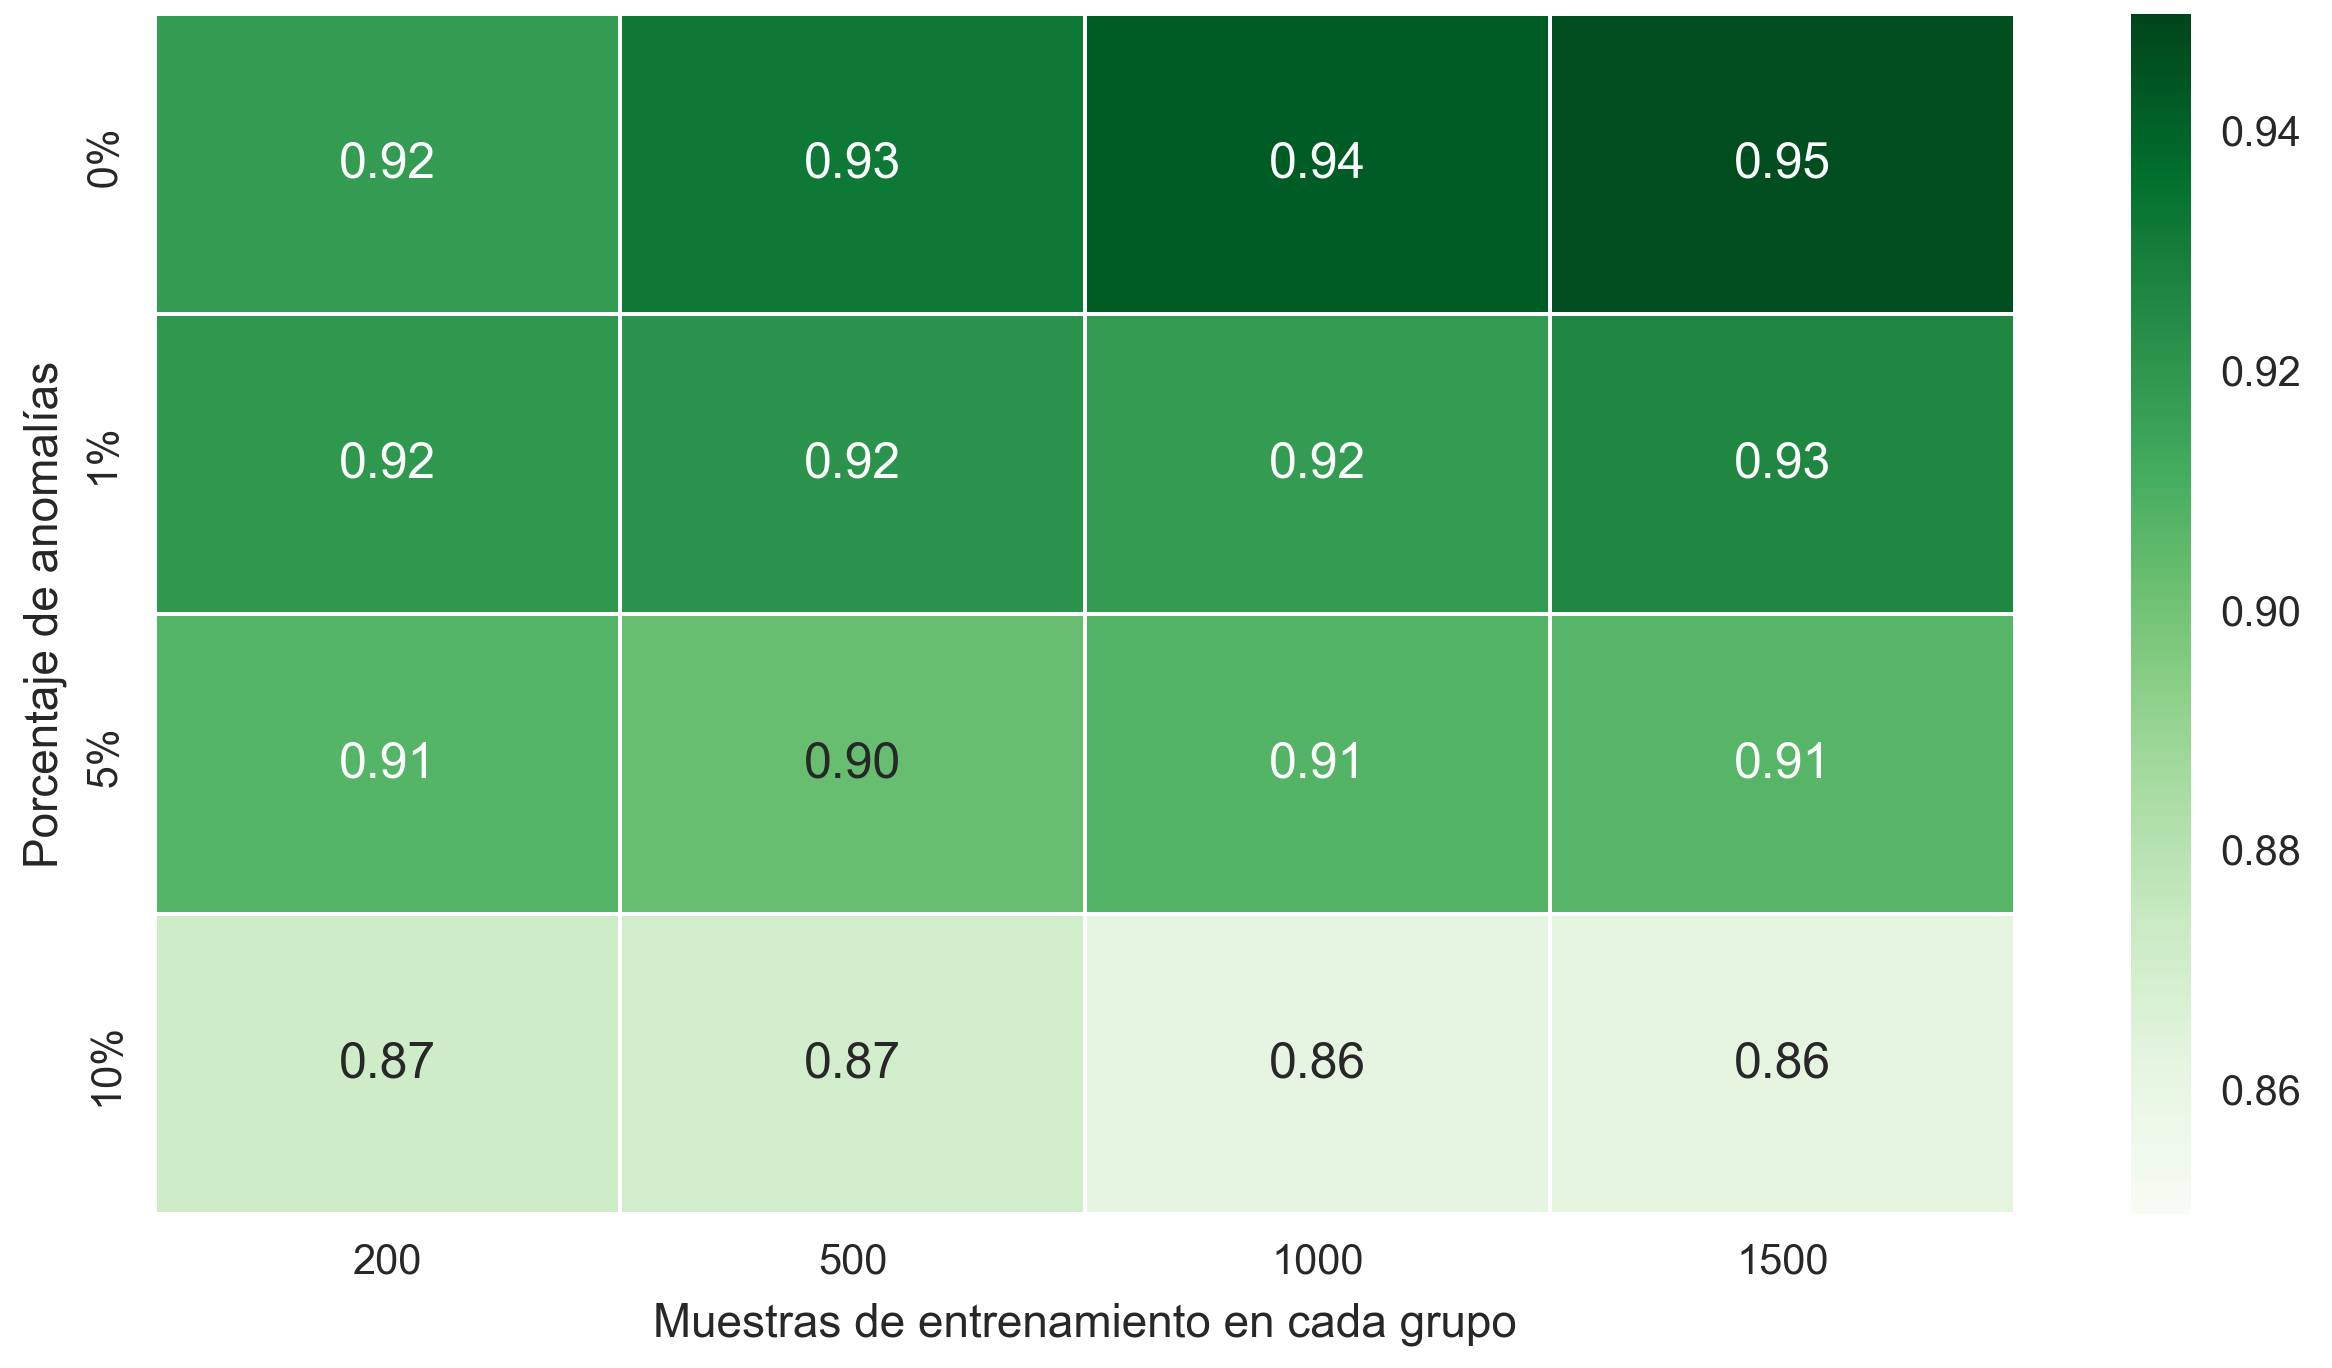
\includegraphics[width=\textwidth]{images/heatmap-results-training-anomalies.png}
    \end{center}
\end{frame}


    \begin{frame}
        \begin{center}
            \small
            \begin{tabular}{c}
                
\includegraphics[height=0.5cm]{images/logo-github.jpg} \\
                \TheRepoUrl \\
            \end{tabular}
        \end{center}
    \end{frame}
\end{document}
